\documentclass[12pt,twoside]{mitthesis}
\usepackage{siunitx}
\usepackage{float}
\usepackage{amsthm}
\usepackage{amsmath, amssymb}
\usepackage{mathtools}
\usepackage{enumerate} 
\usepackage{bm}
\usepackage{dsfont}
\usepackage{times}
\usepackage[round]{natbib}
\usepackage[linktocpage=true]{hyperref}
\usepackage{graphicx}
\usepackage{multirow}
\usepackage{cmap}
\usepackage[T1]{fontenc}
\usepackage[utf8]{inputenc}
\usepackage[margin=1in,footskip=0.25in]{geometry}
\usepackage[bottom]{footmisc}
\raggedbottom
\usepackage{booktabs}
\newcommand{\ra}[1]{\renewcommand{\arraystretch}{#1}}
\renewcommand{\baselinestretch}{1.3}
\usepackage{tikz}

 \usepackage{graphics}
%% or use the graphicx package for more complicated commands
 \usepackage{graphicx}
%% or use the epsfig package if you prefer to use the old commands
%% \usepackage{epsfig}
\usepackage{caption}
\usepackage{subcaption}

\usepackage[acronyms, section, nonumberlist]{glossaries}
\newglossary[slg]{symbolslist}{syi}{syg}{Symbols}
\makeglossaries

\usepackage[toc,page]{appendix}

\hypersetup{
	colorlinks=true, %Colours links instead of ugly boxes
	urlcolor=blue, %Colour for external hyperlinks
	linkcolor=black, %Colour of internal links
	citecolor=red 	 %Colour of citations
}

\clubpenalty=10000			% kara za sierotki
\widowpenalty=10000			% nie pozostawiaj wdĂłw
\brokenpenalty=10000		% nie dziel wyrazów między stronami
\righthyphenmin=3			% dziel minimum 3 litery
\hyphenpenalty=10000

% Theorems
\newtheorem{theorem}{Theorem}[section]
\newtheorem*{remark}{Remark}
\newtheorem{definition}{Definition}[section]
\newtheorem{corollary}{Corollary}[section]
\newtheorem{lemma}{Lemma}[section]

\newcommand{\myparagraph}[1]{\paragraph{#1}\mbox{}\\}


%% Shortcuts
\def\_sp{\left\{X_t, t\in \mathcal{T}\right\}} %% Stochastic process {X_t}
\newcommand{\seqrvs}{X_1, X_2, \ldots, X_n} 	 %% X_1, X_2, ..., X_n
\def\all{all}


\DeclareMathOperator{\spe}{Spec}
\DeclareMathOperator{\Corr}{Corr}
\DeclareMathOperator{\cov}{Cov}
\DeclareMathOperator{\sgn}{sgn}
\DeclareMathOperator{\Var}{Var}
\DeclareMathOperator{\CV}{CV}
\DeclareMathOperator{\scov}{scov}
\DeclareMathOperator{\floc}{FLOC}
\DeclareMathOperator{\flom}{FLOM}
\DeclareMathOperator{\CD}{CD}
\DeclareMathOperator{\ev}{\mathbb{E}}
\DeclareMathOperator{\Z}{\mathbb{Z}}
\DeclareMathOperator{\Prob}{\mathbb{P}}
\DeclareMathOperator{\MSE}{MSE}


\newcommand{\stab}{{$\alpha$-stable }}
\newcommand{\ts}{\{X_t\}_{t\in \mathbb{Z}}}
\DeclareMathOperator{\sign}{sign}
\newcommand{\sas}{{$S \alpha S$}}
\makeatletter
\newcommand{\@giventhatstar}[2]{(#1\,\middle|\,#2)}
\newcommand{\@giventhatnostar}[3][]{#1(#2\,#1|\,#3#1)}
\newcommand{\giventhat}{\@ifstar\@giventhatstar\@giventhatnostar}
\makeatother

% Glosssaries
\renewcommand{\qedsymbol}{$\blacksquare$}

\renewcommand*\acronymname{Abbreviations}
% Abbrevations
\newacronym{iid}{i.i.d.}{independent and identically distributed}
\newacronym{ar1}{AR(1)}{first-order autoregressive process}
\newacronym{cdf}{cdf}{cumulative distribution function}
\newacronym{ecdf}{ecdf}{empirical cumulative distribution function}
\newacronym{pdf}{pdf}{probability density function}
\newacronym{mle}{MLE}{maximum likelihood estimation}

% List of symbols
\newglossaryentry{sp}{
	name={\ensuremath{\left\{X_t, t\in \mathcal{T}\right\}}},
	description={stochastic process},
	sort=symbolStochasticProcess, 
	type=symbolslist
}
\newglossaryentry{f}{
	name={\ensuremath{f(x\,|\,\bm{\theta})}},
	description={probability density function with set of parameters $\bm{\theta}$},
	sort=symbolProbabilityDensityFunction, 
	type=symbolslist
}
\newglossaryentry{GaussianD}{
	name={\ensuremath{\mathcal{N}(\mu,\sigma)}},
	description={Gaussian distribution with mean $\mu$ and standard deviation $\sigma$},
	sort=symbolLevyStableDistribution, 
	type=symbolslist
}
\newglossaryentry{SPRealz}{
	name={\ensuremath{\bm{x}_{1:n}}},
	description={vector of observations, equivalent to $(x_1, x_2, \ldots, x_n)$},
	sort=symbolVectorOfRealization, 
	type=symbolslist
}
\newglossaryentry{randomVector}{
	name={\ensuremath{\bm{X}_{1:n}}},
	description={random vector, equivalent to $(X_1, X_2, \ldots, X_n)^T$},
	sort=symbolVectorOfRealization, 
	type=symbolslist
}
\newglossaryentry{expectedValue}{
	name={\ensuremath{\ev\left(X\right)}},
	description={expected value of random variable $X$},
	sort=symbolExpectedValue, 
	type=symbolslist
}
\newglossaryentry{varianceRV}{
	name={\ensuremath{\Var\left(X\right)}},
	description={variance of random variable $X$},
	sort=symbolVarianceRV, 
	type=symbolslist
}
\newglossaryentry{probEvent}{
	name={\ensuremath{\Prob\left(\mathcal{A}\right)}},
	description={probability of event $\mathcal{A}$},
	sort=symbolProbabilityOfEvent, 
	type=symbolslist
}



\begin{document}
	\begin{titlepage}
	
	\newgeometry{tmargin=1cm,bmargin=1cm,lmargin=2cm,rmargin=2cm}
	
	\begin{center}
		\fontsize{20pt}{25pt}\selectfont
		Wroclaw University of Science and Technology \\
		%\vspace*{.6\baselineskip}
		\fontseries{m}\fontsize{15pt}{15pt}\selectfont
		\textit{Faculty of Pure and Applied Mathematics}\\
		\textit{Department of Applied Mathematics}\\
		
		\vspace*{10\baselineskip}
		\fontseries{m}\fontsize{20pt}{25pt}\selectfont
		Ph.D. Thesis \\
		\vspace*{1.15\baselineskip}
		\fontseries{b}\fontsize{22pt}{25pt}\selectfont
		Modelowanie procesów okresowo skorelowanych z niegaussowskim szumem i ich zastosowanie do diagnostyki technicznej \\
		\vspace*{1.15\baselineskip}
		\fontseries{m}\fontsize{20pt}{15pt}\selectfont
      Piotr Kruczek\\
	\end{center}
	
	\vspace*{6.5\baselineskip}
	\begin{flushright}
		\fontseries{m}\fontsize{13pt}{10pt}\selectfont
		%	Rozprawa doktorska\\
		\textbf{Supervisor:} \\
		\vspace*{0.6\baselineskip}
		dr hab. Agnieszka Wy{\l}oma{\'n}ska, prof. nadzw. PWr\\
	\end{flushright}
	
	\vspace*{6\baselineskip}
	\begin{center}
		\fontseries{m}\fontsize{15pt}{15pt}\selectfont
		\textit{Wroc{\l}aw, \today}
	\end{center}
\end{titlepage}

\pagestyle{empty}
	\cleardoublepage
\pagenumbering{gobble}
\tableofcontents
\cleardoublepage
\pagenumbering{arabic}
	\pagestyle{plain}
	\setcounter{page}{1}
	\chapter{Introduction}
\section{Scope of the thesis}

\newpage
\section{Symbols and annotations}
\glsaddall
\printglossaries
	\chapter{State of the art}\label{chapt:state_of_the_art}

	\chapter{Periodically correlated processes}\label{chapt:PC_process}
\section{Definition}
In the literature, the cyclostationary processes are called also periodically correlated (PC). Their main feature is the periodic structure together with random parts. In particular, the physical process, which contains periodicity and randomness is probably periodically correlated or periodically nonstationary \cite{hurd2007periodically}. This kind of systems are very likely to be observed in many different fields \cite{gardner2006cyclostationarity} e.g. telecommunication \cite{napolitano2016cyclostationarity,wu1996blind}, diagnostics of rotating machinery \cite{randall2001relationship,capdessus2000cyclostationary} or financial data \cite{kruczek2017modified,broszkiewicz2004detecting}. Typically, the second-order PC processes are considered. Given the stochastic process is second-order if its second moment is finite. In this case, there exists a periodic rhythm in the mean and in the autocovariance function. The periodically correlated processes are related to stationary ones, therefore we would like to recall some important definitions \cite{hurd2007periodically}. We are going to consider the probability space $(\Omega,\mathcal{F},P)$ and the stochastic process  $\{X_t(\omega)\}$ (we will use the notation $\{X_t\}$. Moreover, we assume that $t\in \mathbb{Z}$, thus $\{X_t\}$ is called a random sequence (or time series). 
\begin{definition}\label{def1} \cite{hurd2007periodically} Let us consider a random sequence $\{X_t\}$. It is called strictly stationary if for each $n \in \mathbb{Z}$, times $t_1,\dots,t_n\in \mathbb{Z} $ and Borel sets $A_1,\dots ,A_n$ the following holds
\begin{equation}
  P_{t_{1+1},\dots,t_{n+1}}(A_1,\dots,A_n)=  P(X_{t_1+1}\in A_1,\dots ,X_{t_n+1}\in A_n)=P_{t_1,\dots,t_n}(A_1,\dots,A_n).
\end{equation}
\end{definition}
Using the above definition the strictly  periodically stationary random sequence can be introduced.
\begin{definition}\label{def2}\cite{hurd2007periodically}
Let us consider a random sequence $\{X_t\}$. It is called strictly  periodically correlated with period $T \in \mathbb{N}$  if for each $n \in \mathbb{Z}$, times $t_1,\dots,t_n \in \mathbb{Z} $ and Borel sets $A_1,\dots ,A_n$ the following holds
\begin{equation}
    P_{t_{1+T},\dots,t_{n+T}}(A_1,\dots,A_n)=P_{t_1,\dots,t_n}(A_1,\dots,A_n),
\end{equation}
where $T \in \mathbb{Z}$ is the smallest integer in for which the above equation holds. If $T=1$ then this sequence is  strictly stationary.
\end{definition}
In the real applications more often the notion of weakly stationary random sequence is used.  In this case, the second-order random sequences $\{X_t\}\in L^2(\Omega,\mathcal{F},P)$ are used, for which the second moment is finite.  For such sequence, the weak stationarity can be defined.
\begin{definition}\label{def3}
\cite{brockwell2016introduction} Let $\{X_t\}$ be a second-order random sequence. It is weakly stationary if for every $t,h\in \mathbb{Z}$, the following holds
\begin{equation*}
    \ev X_t=m, \quad \cov(X_t,X_{t+h})=\cov(X_0,X_{h}),
\end{equation*}
where $m \in \mathbb{R}$ and $\cov(X_t,X_{t+h})$ is the autocovariance function. Thus, the mean is a constant function and the autocovariance is function depending only on the lag ($h$).
\end{definition}
\begin{definition}\label{def4}\cite{hurd2007periodically,gladyshev}
Let $\{X_t\}$ be a second-order random sequence. It is called periodically correlated with period $T \in \mathbb{N}$ if for every $t,s\in \mathbb{Z}$ the following hold
\begin{equation}
\label{eq:PC def}
    \ev X_{t+T}=\mathbb{E}X_{t}, \quad \cov(X_{t+T},X_{s+T})=\cov(X_{t},X_{s}),
\end{equation}
and $T$ is the smallest number for which the above formulas hold.
\end{definition}
The weakly stationary time series is also PC with period $T$ equal to 1. In the literature, this kind of random sequence is also called second-order cyclostationary.
\section{Analysis}
The cyclic spectral analysis is one of the approach used in the second-order cyclostationary signals analysis.  One of the most powerful tool in this analysis is the  spectral coherence (SC). It is a bi-frequency map, which displays the structure of modulation and carrier frequencies in the signal. 
Firstly, we recall the definition of the cyclic autocorrelation at cycle frequency $\epsilon$ for the sequence $\ts$ \cite{gardner1991exploitation}:
\begin{equation}
    R_X^{\epsilon}(\tau)=\lim_{N\to\infty} \int_{-N/2}^{N/2}R_X(t,\tau)e^{-j2\pi\epsilon t}dt,
\end{equation}
where $\epsilon \in A$ and $A$ is the countable set, not depending on $\tau$, of possible cycle frequencies $\epsilon$ and  $R_X(t,\tau)=\ev X_tX_{t-\tau}$ is the autocovariance function of $\ts$. The values  $R_X^{\epsilon}(\tau)$ are the coefficients of the Fourier expansion of the autocovariance function. 
It was shown in \cite{gardner1978stationarizable} that for  the second-order cyclostationary sequence $\ts$ and for any $t$  $X_t$ and its frequency-shifted version $X_te^{-j2\pi\epsilon t}$ are correlated  for $\epsilon=1/T$.  It means that, random sequence $\ts$ is cyclostationary for cycle frequency $\epsilon$ if $R_X^{\epsilon}(t,\tau)\not\equiv 0$. 
The spectral correlation (cyclic spectrum) at cycle frequency $\epsilon$ is the Fourier transform of the cyclic autocorrelation:
\begin{equation}
    S_X(f,\epsilon)=\int_{-\infty}^{\infty}R_X^{\epsilon}(\tau)e^{-j2\pi f \tau} d\tau.
\end{equation}
And finally the spectral coherence is normalised value of the spectral correlation: 
\begin{equation}
\label{eq:SC}
\left|\gamma_X(f,\epsilon)\right|^{2}=\frac{ \left|S_X(f,\epsilon)\right|^2}{ S_X(f+\epsilon/2,0)S_X(f-\epsilon/2,0)}.
\end{equation}
Therefore, spectral coherence is the double Fourier transform of the instantaneous autocovariance function.
There are many different estimators and algorithms to evaluate the spectral coherence \cite{roberts1991computationally,spooner1994cumulant}. However, in this article the the Avereged Cyclic Periodogram (ACP) \cite{antoni2007cyclic2} is used. In this algorithm, the $S_X(f,\epsilon)$ is estimated by the following value:
\begin{equation}
    S_X^{\textrm{ACP}}(f,\epsilon)=\frac{1}{K||w||^2F_s}\sum_{i=0}^{K-1}X_w(i,f)X_w(i,f-\epsilon)^*,
\end{equation}
where $w(n)$ is a window function and $||w||^2=\sum_{n=0}^{N_w-1}|w(n)|^2$, $N_w$ is length of the window $w(\cdot)$, $K=(L-N_w+R)/R$ is number of windows in signal of length $L$ shifted by $R$ samples, $F_s$ is a sampling frequency and $X_w(i,f)$ is phase corrected STFT defined as \cite{antoni2017fast}:
\begin{equation}
    X_w(i,f)=\sum_{n=0}^{L-1}X_nw(n-iR)e^{-j2\pi iRf/F_s}.
\end{equation} 
It should be mentioned, the main drawback of the ACP-based method is the computational complexity. Therefore, various approaches for more efficient algorithms are studied and developed \cite{antoni2017fast,borghesani2018faster}.
The SC is a perfect tool used for instance in the condition monitoring. Particularly, even for very complicated signals the modulations can be observed based on the cyclic spectrum. SC can be treated as an high-resolution version of envelope spectrum for different carrier frequencies.
\section{Examples}
\label{sec:examples Gaussian}
\subsubsection*{Example 1}
Let us consider the random sequence $\{X_t\}$. It is called periodic, with period $T\in \mathbb{N}$ if for all $t\in \mathbb{Z}$ the following is satisfied 
\begin{equation}
X_{t+T}\overset{d}{=}X_{t},
\end{equation}
and $T$ is the smallest value for which above formula holds. The periodic random sequence is also PC with period $T$.

\subsubsection*{Example 2}
As the second example we consider the sum of a weakly stationary time series and the periodic deterministic function. Let $\{Z_t\}$ be a weakly stationary time series, where $t\in \mathbb{Z}$, $\mathbb{E}Z_t=m$ and $Var(Z_t)=\sigma ^2<\infty$. Moreover, $f(t)$ $f:\mathbb{Z}\rightarrow \mathbb{R}$ is a periodic function with period $T$, i.e. $f(t+T)=f(t)$. Then, the random sequence $\{X_t\}$ defined as
\begin{equation}\label{ex1}
    X_t=f(t)+Z_t, \quad t\in \mathbb{Z}
\end{equation}
is the second-order PC time series. Indeed, we have

\begin{eqnarray}
\ev X_t=f(t)+m=\ev X_{t+T},~~\cov(X_t,X_s)=\cov(Z_t,Z_s)=\cov(Z_{t+T},Z_{s+T})=\cov(X_{t+T},X_{s+T}).\end{eqnarray}
In that case, we observe the periodicity in the mean function of the sequence $\{X_t\}$ as well as in the autocovariance function. The most typical example of the stationary random sequence $\{Z_t\}$ used in equation (\ref{ex1}) is the sequence of Gaussian independent, identically distributed (i.i.d) random variables with zero mean and unit variance.
\subsubsection*{Example 3}
As the third example we consider the product of the weakly stationary time series and the periodic function.  Let $\{Z_t\}$ be the weakly stationary random sequence, where $t\in\mathbb{Z}$, $\mathbb{E}Z_t=m$ and $Var(Z_t)=\sigma ^2<\infty$. Moreover, $f(t)$ $f:\mathbb{Z}\rightarrow \mathbb{R}$ is a periodic function  with period $T$. Then, the random sequence $\{X_t\}$ defined as
\begin{equation}
\label{eq:example3}
    X_t=f(t)Z_t, \quad t\in \mathbb{Z}
\end{equation}
is the second-order PC time series. Indeed, we have
\begin{eqnarray}\ev X_t&=&f(t)m=\ev X_{t+T},\\\cov(X_t,X_s)&=&f(t)f(s)=\cov(Z_t,Z_s)=f(t+T)f(s+T)\cov(Z_{t+T},Z_{s+T})=\cov(X_{t+T},X_{s+T}).\nonumber\end{eqnarray}
The time series defined in (\ref{eq:example3}) is called as amplitude modulation of the stationary time series by the periodic function. As previously, the simplest example of  $\{Z_t\}$ time series in equation (\ref{eq:example3}) is the sequence of  Gaussian i.i.d random variables with zero mean and unit variance.
\subsubsection*{Example 4}
The last considered example is a Periodic Autoregresive Moving Avarage (PARMA)  time series. It is a periodic extension of the well known ARMA (Autoregressive Movin Avarage) time series. The second-order PARMA(p,q) time series is defined as follows \cite{hurd2007periodically,vecchia1985periodic}
\begin{eqnarray}\label{parma1}
X_t-\phi_1(t)X_{t-1}-...-\phi_p(t)X_{t-p}=\xi_{t}+\theta_1(t)\xi_{t-1}+....+\theta_q(t)\xi_{t-q},~t\in \mathbb{Z},
\end{eqnarray}
where the $\{\xi_t\}$ random sequence constitutes sample of i.i.d random variables with mean equal to zero and variance $\sigma^2$. Usually it is assumed that the sequence $\{\xi_t\}$ is Gaussian. The parameter sequences $\{\phi_i(t),~i=1,...,p\}$ and $\{\theta_j(t),~j=1,...,q\}$ are periodic with the same period $T\in \mathbb{N}$ with respect to $t$, i.e. for every $t \in\mathbb{Z}$ the following hold
\begin{eqnarray}
\phi_i(t)=\phi_i(t+T),~\theta_j(t)=\theta_j(t+T),~i=1,...,p,~j=1,...,q.
\end{eqnarray}
We assume that $p,q\in \mathbb{N}$. When $q=0$, the PARMA model is called PAR while when $p=0$ - the PMA model, similar as in the classical ARMA nomenclature \cite{brockwell2016introduction}.
Let us consider the special case of model (\ref{parma1}), namely PAR(1) time series satisfying the following equation
\begin{eqnarray}\label{par1}
X_t-\phi(t)X_{t-1}=\xi_{t},~t\in \mathbb{Z}.
\end{eqnarray}
In that case, the unique bounded (in the sense of $l_2$ norm) solution of equation (\ref{par1}) under the assumption $|\phi(1)\phi(2)...\phi(T)|<1$ is given by \cite{makagon2004bounded}
\begin{eqnarray}\label{par1_rozw}
X_t=\sum_{j=0}^{\infty}\Phi_{t-j+1}^{t}\xi_{t-j},
\end{eqnarray}
where $\Phi_{k}^n=\prod_{r=k}^n\phi(r)$ with the convention $\Phi_k^n=1$ when $k>n$, see also \cite{nowicka2006dependence}.\\
Let us assume $s,t \in \mathbb{Z}$, $s>t$. Moreover, for the simplicity let  the $\{\xi_t\}$ sequence constitutes the sample of zero mean and unit variance. 
Using (\ref{par1_rozw})  we obtain
\begin{eqnarray}\ev (X_t)&=&0=\ev (X_{t+T})\\
\ev (X_sX_t)&=&\sum_{j=0}^{\infty}\left(\Phi_{t-j+1}^t\right)^2\Phi_{t+1}^s=\sum_{j=0}^{\infty}\left(\Phi_{t+T-j+1}^{t+T}\right)^2\Phi_{t+T+1}^{s+T}=\ev (X_{s+T}X_{t+T}).\nonumber\end{eqnarray}
Thus, PAR(1) time series given in (\ref{par1}) under the considered assumptions is the second-order PC sequence. In general, under some assumptions, the PARMA(p,q) model defined in (\ref{parma1}) is a second-order PC time series. It is worth to mention, for $T= 1$ the PARMA time series  is reduced to the  ARMA model \cite{brockwell2016introduction}.
The explicit form for the solution and spectral analysis for PARMA sequence are presented in \cite{wylomanska2008spectral}.
	\chapter{$\alpha$-stable distribution and processes}\label{chapt:stable}
\section{Definition of \stab distribution}
One of the most common generalization of Gaussian distribution is the $\alpha-$stable one.  It was introduced by Paul L{\'e}vy and Aleksander Khinchine in the 1920s and 1930s \cite{levy1924theorie,khinchine1936lois}.
The $\alpha$-stable random variable is described by four parameters: stability index $\alpha$, the scale parameter $\sigma$ (it is called as well the dispersion), skewness parameter $\beta$ and shift parameter $\mu$.    
 In the literature, one can find many different equivalent definitions of this distribution. It is worth mentioning that the closed form of the probability density function typically does not exist (only for particular cases). However, the characteristic function is given, thus one of the most popular definition of the \stab random variable can be formulated in the language of the characteristic function.
\begin{definition}
\label{def6}\cite{stable}
Let $X$ be a random variable, it follows the \stab distribution ($X\sim S(\alpha,\sigma,\beta,\mu)$) if its characteristic function has the following form:
\begin{eqnarray}\label{chf_1}
\phi_X(t)=\mathbb{E}e^{itX}=\left\{
\begin{array}{ll} 
\exp\left\{-\sigma^{\alpha}|t|^{\alpha}\left(1-i\beta\sgn(t)\tan\left(\frac{\pi\alpha}{2}\right)\right)+i\mu t\right\} & \alpha\neq 1,\\
&\\
\exp\left\{-\sigma|t|\left(1+i\beta\,\frac{2}{\pi} \sgn(t)\ln\left(|t|\right)\right)+i\mu t\right\} & \alpha = 1,
\end{array}\right.
\end{eqnarray}
where parameters $\alpha \in (0,2]$, $\beta \in [-1,1]$, $\sigma>0$ and $\mu \in \mathbb{R}$. 
\end{definition}
For $\alpha<2$, the  second moment (and thus the variance) of $X$ does not exist. Moreover, for $\alpha<1$ even the mean is infinite. On the other hand, the Gaussian distribution belongs to the class of $\alpha$-stable distributions. In case of stability index equal to $\alpha=2$ and skewness parameter $\beta =0$, the $\alpha-$stable distribution reduces to the Gaussian one. 

The $\alpha$ parameter is related to the so-called heavy-tailed property of the distribution. Indeed, the smaller $\alpha$  the larger values of a random variable $X$ can be obtained.
In particular, the stability index is responsible for the rate of the distribution tail decay. For $\alpha<2$ the \stab distribution exhibits a power-law behaviour \cite{stable}:
\begin{eqnarray}\label{eq:power}
\left\{ 
\begin{array}{ll} 
\lim_{x\to\infty} x^{\alpha}P\{X>x\}=C_{\alpha}\frac{1+\beta}{2}\sigma^\alpha,\\
&\\
\lim_{x\to{}\infty} x^{\alpha}P\{X<-x\}=C_{\alpha}\frac{1-\beta}{2}\sigma^\alpha,
\end{array}\right.
\end{eqnarray}
where $C_{\alpha}=\left(\int_0^{\infty}x^{-\alpha}\sin(x)dx\right)^{-1}=\frac{1}{\pi} \Gamma (\alpha)\sin (\frac{\pi \alpha}{2})$ and $\Gamma(\cdot)$ is a Gamma function.

In this paper we concentrate on the special case of the large class of \stab distribution, namely we take under consideration the symmetric $\alpha$-stable distribution (further denoted as $S\alpha S$).
\begin{definition}
\label{def7}\cite{stable}
The random variable $X$ has $S\alpha S$ distribution ($X\sim S\alpha S(\alpha,\sigma)$) with scale parameter $\sigma$ and stability index $\alpha$ if the characteristic function of $X$  is given by:
\begin{eqnarray}\label{char}
\phi_{X}(t)=\ev\exp(itX)=\exp(-\sigma^{\alpha}|t|^{\alpha}).
\end{eqnarray}
\end{definition}
Through the \stab random signal we understand the 
time series $\ts$, $t\in \mathbb{Z}$ such that for each $t~~X_t\sim S\alpha S(\alpha,\sigma)$.
One of the problem of analysing the $\alpha-$stable-based processes follows from the fact that there exist many types of them. For each type we have different properties.  However, there are three types of the \stab random systems that are most often considered in practice: sub-Gaussian processes \cite{cambanis_soltani}, linear $\alpha-$stable processes \cite{kluppelberg1993spectral,klup1994,klup1995,klup1996,nw1,nowicka2006dependence} and harmonizable $\alpha-$stable processes \cite{cambnnis1981linear,weron1985,makagon_mandrekar1990}, see also \cite{shao,stable}.

It is important to highlight that, for the finite-variance time series the classical measure of dependence is the autocovariance (or autocorrelation) function. However, when we consider the \stab random signal  with $\alpha<2$, the classical autocovariance function is infinite, thus it should not be used to analyze the dependence structure of the time series. Therefore, another measures of dependence are used in this case. In the literature, several different measures are introduced and compared \cite{cambanis1980some,stable,rosinski1997equivalence,kodia2014estimation,damarackas2014properties}. In case of $\alpha$-stable distribution typically the second moment does not exist, however one can consider the fractional lower order moments (FLOM). FLOM is one of the most popular statistics for \stab random variables. Let $X$ be a random variable, the $\flom$ of order $0<p<2$ is  defined as:
\begin{equation*}
    \flom(X,p)=\ev|X|^p.
\end{equation*}

If $X$ is the \stab random variable, then the FLOM exist for all orders $p<\alpha$. Therefore, this statistic, with particular order $p$, is finite and well-defined for \stab distribution. For the \sas random variable one can found the relation between the dispersion and FLOM, namely
 \cite{stable}:
\begin{equation*}
    \textrm{FLOM}(X,p)=C(p,\alpha){\sigma^{\frac{p}{\alpha}}} \quad \textrm{for } 0<p<\alpha,
\end{equation*}
where 
\begin{equation*}
    C(p,\alpha)=\frac{2^{p+1}\Gamma(\frac{p+1}{2})\Gamma(\frac{-p}{\alpha})}{\alpha\sqrt{\pi}\Gamma(\frac{-p}{2})}.
\end{equation*}
%%%%%%%%%%%%%%%%%%%%%%%%%%%%%%%%%%%%%%%%%%%%%%%%%%%%%%%%%%%%%%%%%
%
%%%%%%%%%%%%%%%%%%%%%%%%%%%%%%%%%%%%%%%%%%%%%%%%%%%%%%%%%%%%%%%%%
\subsection{Examples}
%%%%%%%%%%%%%%%%%%%%%%%%%%%%%%%%%%%%%%%%%%%%%%%%%%%%%%%%%%%%%%%%%
%
%%%%%%%%%%%%%%%%%%%%%%%%%%%%%%%%%%%%%%%%%%%%%%%%%%%%%%%%%%%%%%%%%
\section{Alternative measures of dependency}
%%%%%%%%%%%%%%%%%%%%%%%%%%%%%%%%%%%%%%%%%%%%%%%%%%%%%%%%%%%%%%%%%
%
%%%%%%%%%%%%%%%%%%%%%%%%%%%%%%%%%%%%%%%%%%%%%%%%%%%%%%%%%%%%%%%%%
\section{Definition of \stab processes}
\subsection{The $\alpha-$stable autoregressive models}
The autoregressive-moving average (ARMA) time series are very often used to description of different empirical processes. In classical version the ARMA(p,q) time series is defined as follows \cite{brockwell2016introduction}:
\begin{eqnarray}\label{arma1}
X_t-\phi_1X_{t-1}-...-\phi_pX_{t-p}=\xi_t+\theta_1\xi_{t-1}+...+\theta_q\xi_{t-q},~t\in \Z,
\end{eqnarray}
where $\{\xi_t\}$ is a white noise sequence with mean zero and variance equal to $\sigma_{\xi}^2$. The $p$ parameter is the order of autoregression while the $q$ parameter - the order of moving average part. Equation (\ref{arma1}) can be written in equivalent form:
\begin{eqnarray}\label{arma2}
\Phi(B)X_t=\Theta(B)\xi_t,
\end{eqnarray}
where $\Phi(z)=1-\phi_1z-...-\phi_pz^p$ and $\Theta(z)=1+\theta_1z+...+\theta_qz^q$ are polynomials of autoregressive and moving-average parts, respectively. Moreover, $B$ is the backward shift operator, namely $BX_t=X_{t-1}$.  It is also assumed the polynomials $\Phi(z)$ and $\Theta(z)$ have no common roots. In the classical time series literature the $\xi_t$ for each $t$ is either Gaussian or non-Gaussian with finite variance. Therefore the probability that it can take large values is very small. In this paper we focus only on the AR(p) time series that satisfies equation (\ref{arma2}) with $\Theta(z)=1$. Moreover, instead of finite variance sequence $\{\xi_t\}$ we assume the noise constitutes sequence of iid random variables with $S\alpha S$ distribution, i.e. for each $t$, the random variable $\xi_t$ has the characteristic function given in equation (\ref{char}) for some parameters $1<\alpha\leq 2$ and $\sigma_{\xi}>0$. Under above presented assumptions it is proved in \cite{stable} that the system satisfying equation (\ref{arma2}) has a unique solution of the form:
\begin{eqnarray*}\label{sol}
X_t=\sum_{j=0}^{\infty}c_j\xi_{t-j}, ~t\in \Z,~a.s.
\end{eqnarray*}
with real $c_j$'s satisfying $|c_j|<Q^{-1}$ where $Q>1$, if and only if $\Phi(z)$ has no roots in the unit disc $\{z:~|z|\leq 1\}$. The sequence $\{X_t\}$ is then a stationary process and has $S\alpha S$ distribution. The parameters $c_j$'s are coefficients in the series expansion $\Theta(z)/\Phi(z)$ for $|z|<1$.

In \cite{nowicka1} the asymptotic behavior of the autocovariation as well as the autocodifference for ARMA(p,q) system with $S\alpha S$ distribution is shown. It is worth mentioning that the main result of \cite{nowicka1} is the fact that the ratio $CD(X_{t+k},X_t)/CV(X_{t+k},X_t)$ for large values of $k$ parameter tends to $\alpha$. \\
For the special case, namely for AR(1) time series given by the equation:
\begin{eqnarray*}\label{ar1}
X_t-\phi X_{t-1}=\xi_t,
\end{eqnarray*}
where $|\phi|<1$ and $\{\xi_t\}$ is a sequence of iid $S\alpha S$ random variables with $\alpha>1$ and $\sigma_{\xi}>0$, one can obtain the exact formulas for autocovariation and autocodifference \cite{nw1}
\begin{eqnarray*}
\label{ar1_cd}CV(X_{t+k},X_{t})=\frac{\sigma_{\xi}^\alpha |\phi|^k}{1-|\phi|^\alpha},\\
CV(X_t,X_{t+k})=\frac{\sigma_{\xi}^\alpha |\phi|^{\alpha k}}{\phi^k(1-|\phi|^\alpha)},\\
CD(X_{t+k},X_t)=\frac{\sigma_{\xi}^{\alpha}(1+|\phi|^{k\alpha}-|1-\phi^k|^{\alpha})}{1-|\phi|^{\alpha}}.
\end{eqnarray*}
\subsection{The $\alpha-$stable periodic autoregressive models}
Conventional time-series analysis is heavily dependent on the assumption of stationarity. But this assumption is unfulfilled for many physical processes of interest. Periodically correlated (PC) processes offer an interesting alternative. They are non-stationary but possess many stationary processes properties. Hence, one can find the numerous attempts to apply PC processes in various areas of science and technology \cite{broszkiewicz2004detecting}. The second-order PC time series $\{X_t\}$ is a process for which the mean as well as the covariance functions are periodic with the same period $T$, more precisely:
\begin{eqnarray*}
\label{eq:periodicity}
\ev(X_{t})=\ev(X_{t+T}),~~ACVF(X_{t+k},X_t)=ACVF(X_{t+T+k},X_{t+T}).
\end{eqnarray*}
As McLeod \cite{mcleod1993parsimony} observes, periodically correlated series should not be modelled with,
the widely used in econometrics, seasonal autoregressive moving-average (SARMA) class.  A flexible group of models that posses the desirable properties is the class
of periodic autoregressive moving-average (PARMA) models. Analogous to ARMA systems and short memory stationary series, second-order PARMA models are fundamental periodiccite{nowi}
and periodically correlated time series models \cite{vecchia1985periodic,ghysels2001econometric,lund2000recursive}.\\
The classical second-order PARMA(p,q) is defined through the following equation:
\begin{eqnarray}\label{parma1}
X_t-\phi_1(t)X_{t-1}-...-\phi_p(t)X_{t-p}=\xi_{t}+\theta_1(t)\xi_{t-1}+....+\theta_q(t)\xi_{t-q},
\end{eqnarray}
where, similar as for ARMA model, the $\{\xi_t\}$ sequence constitutes an iid sample of uncorrelated random variables with mean equal to zero and variance $\sigma_{\xi}^2$. Usually it is assumed that the sequence $\{\xi_t\}$ is a Gaussian white noise. The scalar sequences $\{\phi_i(t),~i=1,...,p\}$ and $\{\theta_j(t),~j=1,...,q\}$ are periodic in $t$ with the same period $T$. Clearly, for $T= 1$ the PARMA time series  is reduced to classical ARMA system defined in (\ref{arma1}). We should mention, the PARMA models are special case of time-varying ARMA systems for which the coefficients depend on time \cite{nw1}.\\
In this paper we analyse the special case of time series (\ref{parma1}), namely PAR(p) model defined as:
\begin{eqnarray}\label{eq:PAR}
X_t-\phi_1(t)X_{t-1}-...-\phi_p(t)X_{t-p}=\xi_{t}.
\end{eqnarray}
It is worth mentioning that the second-order PAR models are associated with the vector AR time series and there is one to one correspondence between such two systems \cite{wylomanska2008spectral,hurd2007periodically}.\\
For many real data, which exhibit behavior related to periodically correlated processes, the assumption of Gaussian or another finite variance distribution seems to be inadequate. Therefore, in the literature there are considered PAR models with heavy tailed distributions, like $\alpha-$stable \cite{nowicka2006dependence}. The PAR model with $\alpha-$stable innovations satisfies equation (\ref{eq:PAR}) with periodic coefficients $\{\phi_i(t),~i=1,...,p\}$. However, in contrast to the classical PAR system, the sequence $\{\xi_t\}$ constitutes sample of iid random variables with $S\alpha S$ distribution, i.e. for each $t$, the random variable $\xi_t$ has the characteristic function given in (\ref{char}). In this case the PC property can not be expressed by autocovariance function but by means of alternative measures of dependence, like autocovariation or autocodifference.

For the special case, namely for PAR(1) system with $\alpha-$stable distribution and period of length $T$:
\begin{eqnarray*}
X_t-\phi(t)X_{t-1}=\xi_t
\end{eqnarray*}
under the assumption $1<\alpha \leq 2$, $\sigma_{\xi}>0$ and $|P|=|\phi(1)...\phi(T)|<1$, the autocovariation and autocodifference take the forms \cite{nowicka2006dependence}:
\begin{eqnarray*}
\label{par1_cd}CV(X_{n+k},X_{n})=\frac{\sigma_{\xi}^{\alpha}B_{n+1}^{n+k}}{1-|P|^{\alpha}}\sum_{j=0}^{T-1}|B_{n-j+1}^n|^{\alpha},\\
CV(X_n,X_{n+k})=\frac{\sigma_{\xi}^{\alpha}}{B_{n+1}^{n+k}(1-|P|^{\alpha})}\sum_{j=0}^{T-1}|B_{n-j+1}^{n+k}|^{\alpha},\\
CD(X_{n+k},X_n)=\sigma_{\xi}^{\alpha}\frac{1+|B_{n+1}^{n+k}|^{\alpha}-|1-B_{n+1}^{n+k}|^{\alpha}}{1-|P|^{\alpha}}\sum_{j=0}^{T-1}|B_{n-j+1}^n|^{\alpha},
\end{eqnarray*}
where for $i\geq j$  $B_{i}^{j}=\phi(i)...\phi(j)$. What is interesting, similarly as for $\alpha-$stable ARMA systems, it can be also shown that for PAR(1) time series with $\alpha-$stable innovations the ratio $CD(X_{n+k},X_n)/CV(X_{n+k},X_n)$ for large values of $k$ parameter tends to $\alpha$ \cite{nw2}.
\subsection{Examples}
\section{Multivariate \stab distribution and processes}
	 \chapter{Cyclostationary \stab processes}\label{chap::cyclo_stab}
\section{Definition}
\section{Examples}
	\chapter{New methods for analysis cyclostationary \stab processes}\label{chap::new_methods}
\section{Time domain methods}
\subsection{The modified Yule-Walker method for \stab time series}
\subsubsection{Covariation based method}
\subsubsection{FLOC based method}
\section{Spectral methods}
\subsection{Cyclic sources extraction from complex multiple-component vibration signal via periodically time varying filter}
\label{sec:semi_blind_methodology}
The proposed methodology consists of six main steps. In the first one the vibration signal $x(t)$ is converted into the time-frequency domain. In this paper we propose to use the spectrogram, which is based on the short-time Fourier transform, although other decompositions might be beneficial as well. The formula for spectrogram is presented in equation~(\ref{eq:spectrogram}): 
\begin{equation}
\label{eq:spectrogram}
\begin{gathered}
\spe(t,f)=\left|STFT(t,f)\right|^2
=\left|\sum_{m=0}^{K-1}w(t-m)x(m)e^{-2i\pi fm/K}\right|^2,
\end{gathered}
\end{equation}
where $w(\cdot)$ is a $W$-long window function, $t=1,\ldots,N$ is a time point, $f$ is a frequency bin and $K\geq M$ is the number of points in which the Fourier Transform is calculated. Given the time-frequency representation of the data, time series related to each frequency bin are examined for having cyclic properties. Periodic amplitude modulation, shared by several frequency bins, might be a signature of local damage.  It starts with spectrogram-based decomposition of the signal on subbands with following parameters:  $N_w$ - window length, $Ov$ - overlap (percentage of overlapping windows), $fs$ - sampling frequency and $NFFT$ - the number of FFT points. In the next step the analyzed fault frequency has to be set. In case of testing several different fault frequencies the following operation have to be repeated for each fault frequency separately. Thus, the proposed methodology allows to extract separate sources related to different modulation frequencies. On the other hand, indicators of the informative frequency band, e.g. spectral kurtosis, infogram, protrugram etc. would indicate both carrier frequency bands as containing information about local damage \cite{antoni2006spectral,barszcz2011novel,antoni2016infogram,obuchowski2014selection}. As a result, signals related to each fault frequency would not be separated.
\begin{figure}[ht!]
\centering
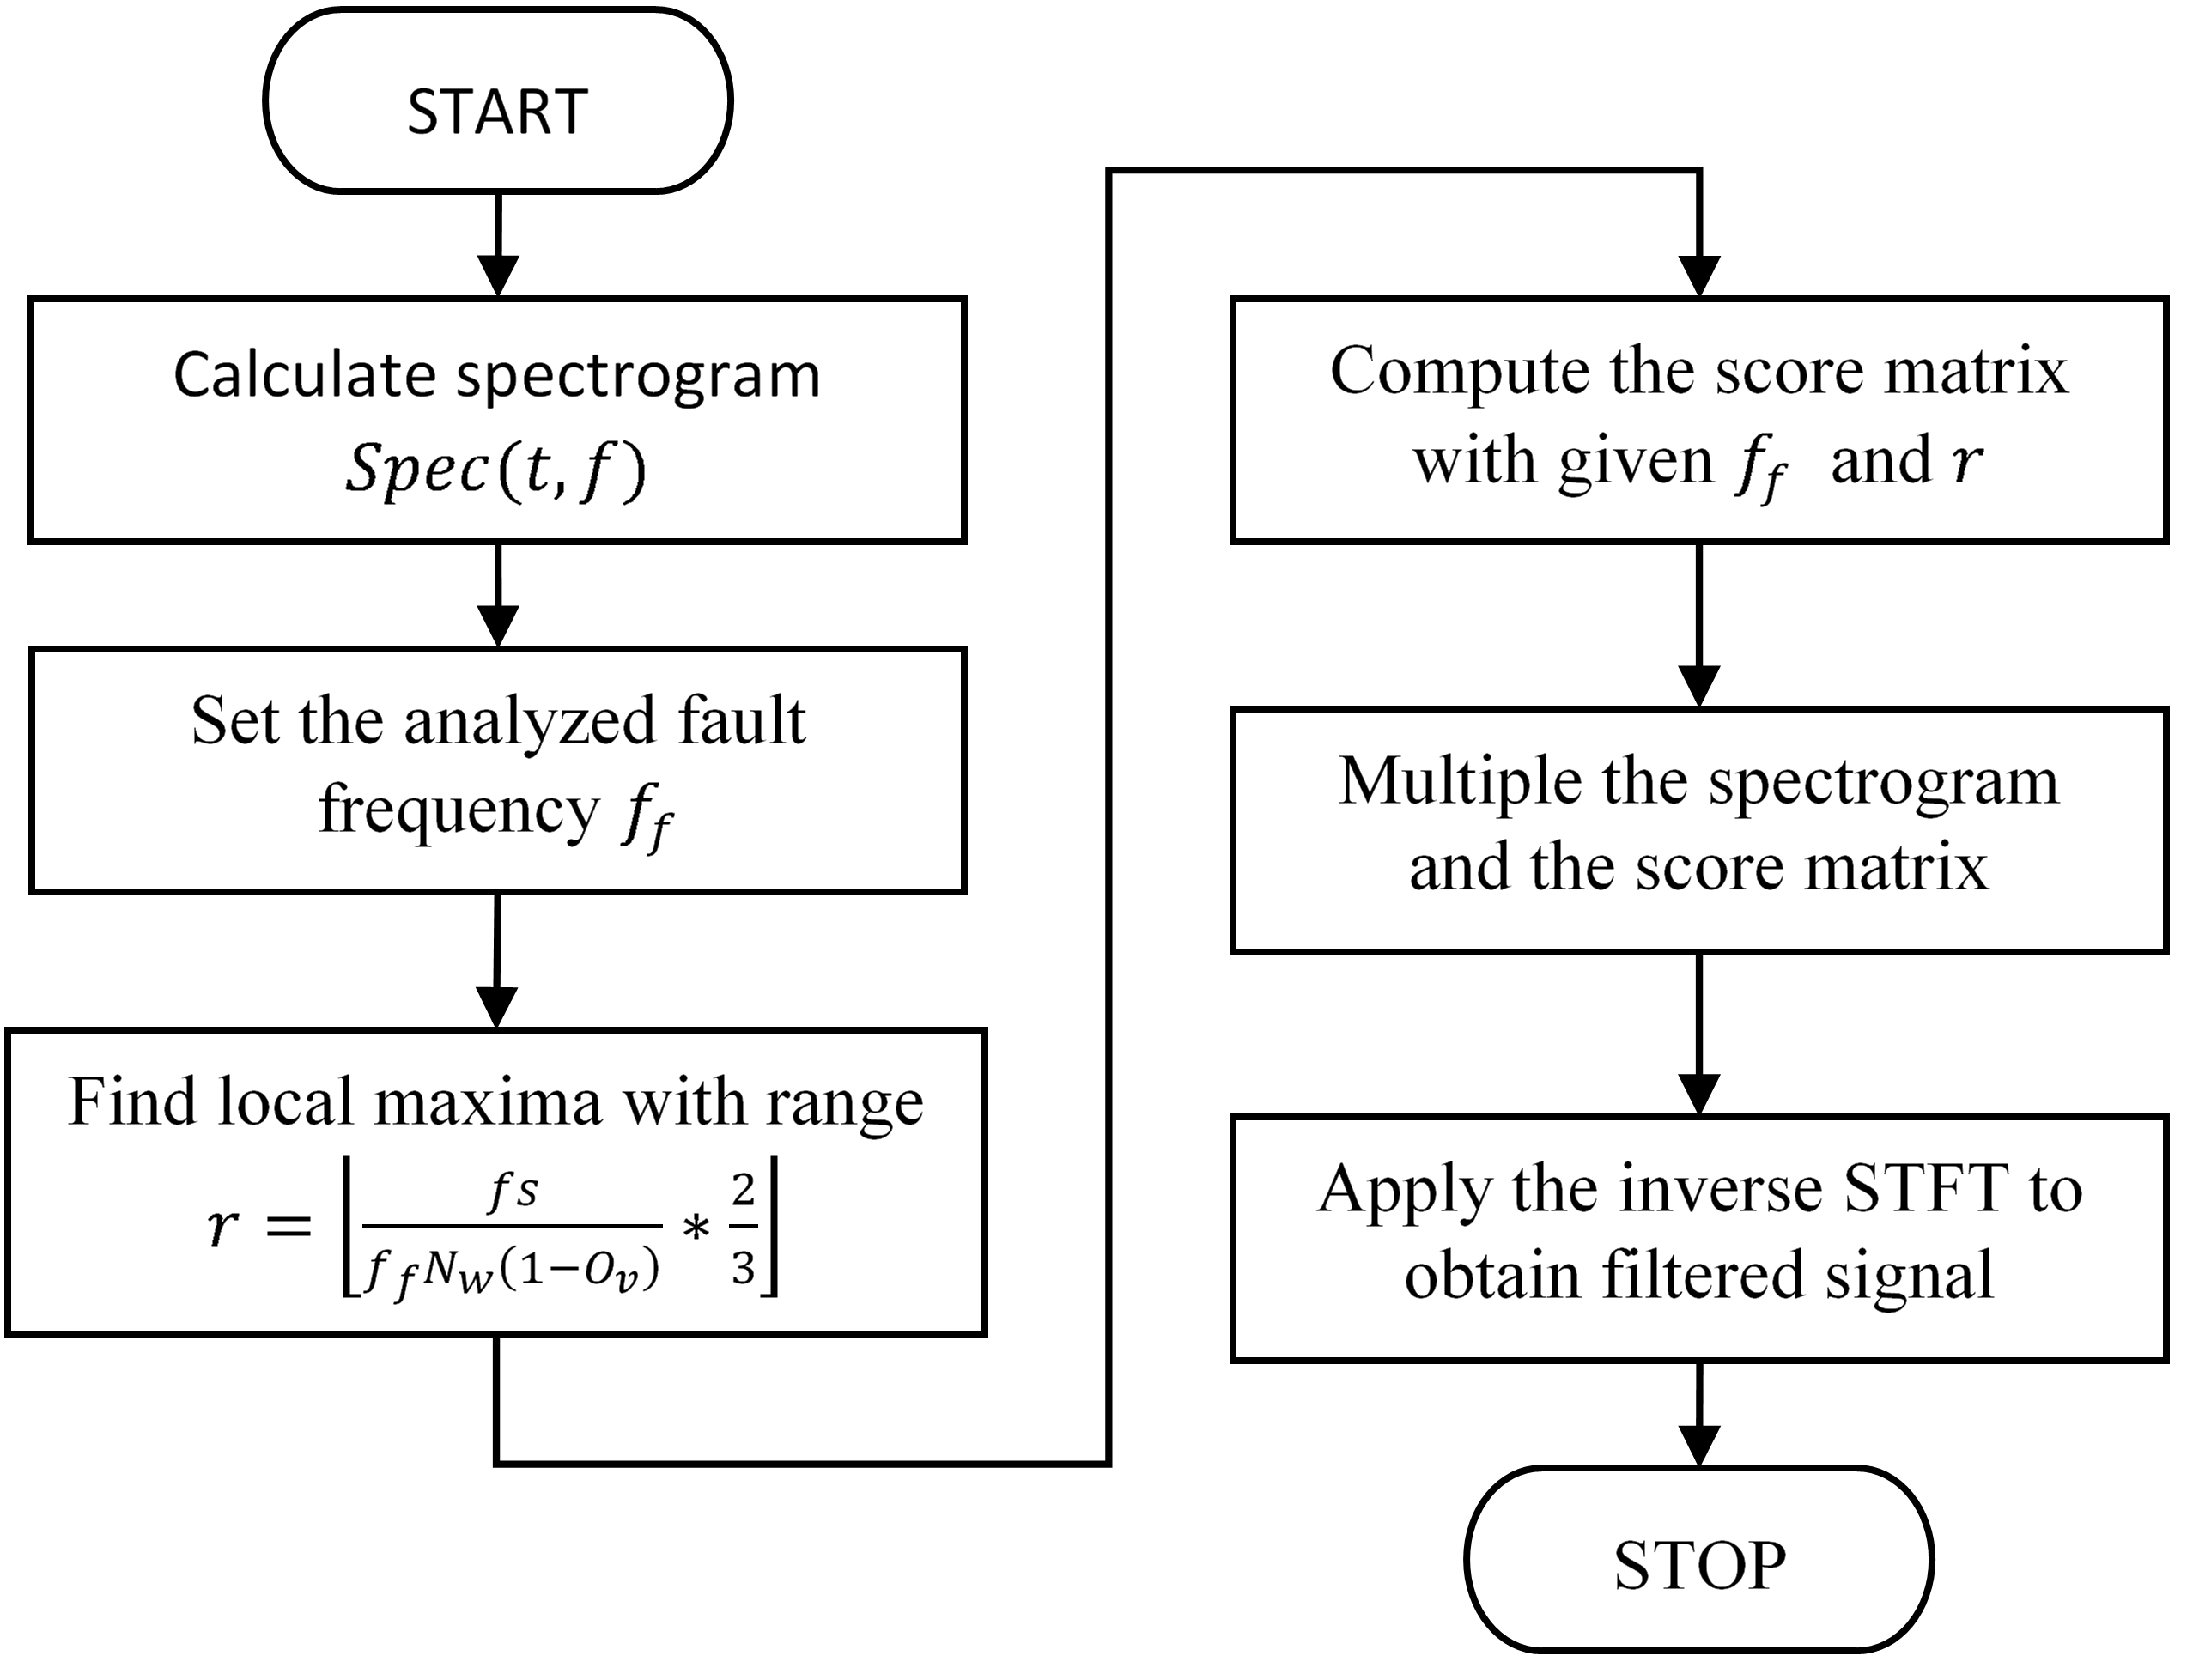
\includegraphics[width=0.8\textwidth]{wykresy/chapter_new_methods/semi_blind/algorytm_blind_source_extraction.png}
\caption{Flowchart of the semi-blind  source extraction algorithm.}
\label{fig:semi-blind algorytm}
\end{figure}


In the following step for each frequency bin in the time series $\spe(:,f)$ local maxima are found. The crucial parameter in this step is the range in which the maximum is founded. Low range leads to large number of local maxima unrelated to local damage. On the other hand, wide range could result in some significant fault signatures omitted. Therefore, we propose to relate the range with considered fault frequency, i.e. $r=\left\lfloor \frac{2}{3}\frac{fs}{f_f N_w(1-O_v)}\right\rfloor$. Such $r$ translates the period related to fault frequency into the spectrogram time axis. The factor $\frac{2}{3}$ is responsible for slight reduction of the range, since subsequent fault-related local maxima might occur on the boundary of the period $1/f_f$. The binary function that indicates if the time point $t_i$ reveals the local maximum might be defined as:
\begin{displaymath}
M(t_i,f)= \left\{ \begin{array}{ll}
1, & \quad \text{if } \spe(t_i,f)=\max_{i-r\leq k \leq i+r}\left\{\spe(t_k,f)\right\} 
\\ 
0, & \quad \text{otherwise.}
\end{array}
\right.
\end{displaymath}
Thereafter each subband in $M$ is considered separately. Given $f$, a score, which quantifies periodicity, is assigned to each $t_i$. It evaluates the average of $M$ values at time points $(\ldots,t_{i}-2T,t_{i}-T,t_i,t_{i}+T,t_{i}+2T,\ldots)$, namely: 
$$
score(t_i,f)=\frac{\sum_{1 \leq t_i + kT \leq \lfloor N/T\rfloor}M(t_i+kT,f)}{\lfloor N/T\rfloor},
$$
where $T=\left\lfloor \frac{fs}{f_f N_w(1-O_v)}\right\rfloor$ is the fault-related period (in samples) and $k\in \mathbb{Z}$. The score matrix indicates the average number of local maxima in time points spaced by $T$. Thus, it might be considered as a time-varying filter with periodic coefficients, since $score(t_i,f)=score(t_i + kT,f)$.\\
In order to return to the time domain the STFT is multiplied element-wise by the score matrix. Then, the inverse short-time Fourier transform algorithm is applied to such STFT with modified amplitudes and filtered signal $y(t)$ might be further analyzed~\cite{boashash2015time}:
$$
y(t)=\int_{-\infty}^\infty\int_{-\infty}^\infty STFT_x(t,f)score(t,f)e^{2\pi i ft}dt df.
$$
%
The numerical computation of the inverse short-time Fourier transform can be applied with weighted Overlap-add method~\cite{dutoit2010applied}. As the result both the filtered and raw signals are of the same length. Amplitude of $y(t)$ reflects not only presence of periodic local maxima in raw signal spectrogram but also real amplitudes related to them. Thus, the proposed method takes into account presence of periodic amplitude modulation in each subband separately, and the corresponding energy. It is worth mentioning that in case of real signal, which is cyclostationary of order 2 (CS2), $y(t)$ is also CS2. Therefore, the standard envelope based method can be applied. On the other hand, proposed filtration provide the signal, which contain only the cyclic components, thus the proper harmonics should be more visible in the envelope spectrum. In Fig.~\ref{fig:semi-blind algorytm} the flowchart of the proposed algorithm is presented. 

Clearly, real signals might consist of two sources with different modulation frequencies, which are observed in different carrier frequencies. In most of such cases the algorithm is expected to separate signal sources appropriately. The problem might occur once the first modulation frequency is the multiple of the second and related series of excitations are consistent in phase. The extracted signal related to the lower modulation frequency would contain some of the excitations related to the higher modulation frequency. This problem can be overcome with the proper local maxima range $r$ selection. It is worth mentioning that once the range $r$ value is too high for given fault frequency, the periodic local maxima would not be detected. One can observe that it is of great importance to set the proper $r$. It is also of high importance if the proposed methodology requires pre-whitening in order to appropriately deal with high-energy components.
\subsection{A}
	\chapter{Application for local damage detection}\label{chap:application}
\section{Application for simulated data}
\subsection{Cyclic sources extraction from complex multiple-component vibration signal via periodically time varying filter}
Firstly, the methodology introduced in Section~\ref{sec:chapter7/semi_blind/schemat_przekladniasemi_blind_methodology} is applied to the simulated data. Such application gives a possibility to check if the algorithm performs appropriately for the entirely known signal. We would like to analyzed three cases. In particular, first one consists of two different components corresponded to the fault. In order to test the performance in case of variable period of the damage the signal with jitter is simulated. Finally, in the last case the signal without any cyclic component is analyzed with proposed method. It would inform how the proposed method is sensitive for the false alarm.

\subsubsection{Signal with multiple fault source}
\label{sec:chapter7/semi_blind/schemat_przekladniamultiple source_semi_blind}
Let us analyse firstly the signal with multiple cyclic components. It corresponds to the machine, in which two damages occur. One can be interested if the method is able to extract both cyclic components.
The length of the signal is 2.5 seconds and the sampling frequency is  8192~Hz. The signal is presented in time and time-frequency domain in Fig.~\ref{fig:chapter7/semi_blind/time-plot_sim}.
\begin{figure}[!ht]
    \centering
    \begin{subfigure}[b]{0.8\textwidth}
        \centering
        \captionsetup{skip=0.01pt}
         \caption{}
        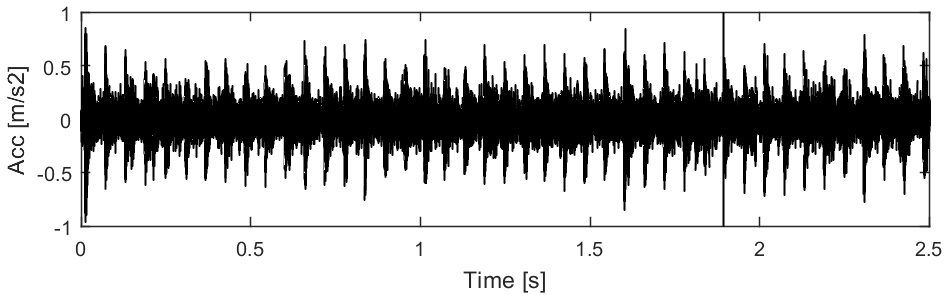
\includegraphics[width=\textwidth]{wykresy/chapter_application/semi_blind/sygnal_simulated.png}
        % \label{fig:chapter7/semi_blind/time_sim}
    \end{subfigure}
    %\hfill
    \begin{subfigure}[b]{0.7\textwidth}
        \centering
        \captionsetup{skip=0.01pt}
         \caption{}
        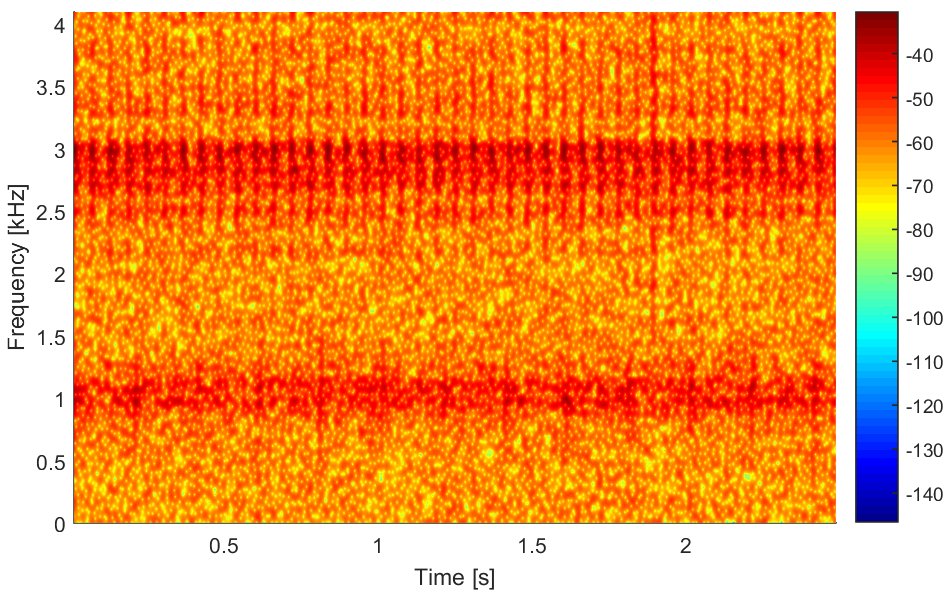
\includegraphics[width=\textwidth]{wykresy/chapter_application/semi_blind/spectrogram_simulated.png}
        % \label{fig:chapter7/semi_blind/spectrogram_sim}
    \end{subfigure}
%    \hfill
    \begin{subfigure}[b]{0.8\textwidth}
        \centering
        \captionsetup{skip=0.01pt}
        \caption{}
        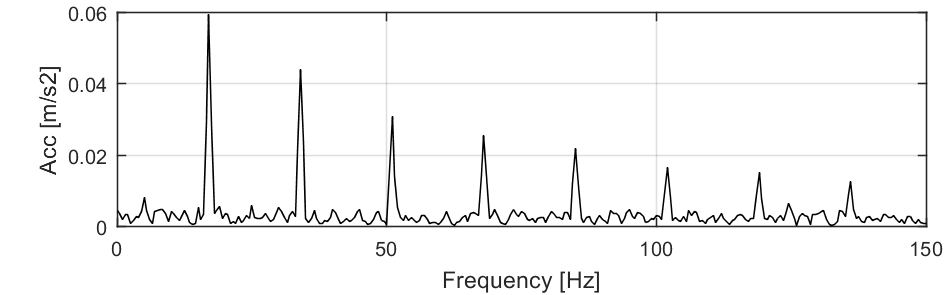
\includegraphics[width=\textwidth]{wykresy/chapter_application/semi_blind/widmo_obwiedni_simulated.png}
        \label{fig:chapter7/semi_blind/obwiednia_sim}
    \end{subfigure}
    \caption{Time plot (a), spectrogram (b) and envelope spectrum (c) of the vibration simulated signal with two damages. The spectrogram parameters are as follows: $N_w=250$, $Ov=96\%$.}
    \label{fig:chapter7/semi_blind/time-plot_sim}
\end{figure}
\\
There are two periodic impulse trains with modulation frequencies 5~Hz and 17~Hz, respectively, and random noise added to each pulse train. Corresponding time plots are presented in Fig.~\ref{fig:chapter7/semi_blind/sim_skladowe}, where periodic impulses can be observed. These components represent local fault, which can occur in a rotating machine. The carrier frequency bands are 700-1300~Hz and 2300-3200~Hz for modulation frequencies 5~Hz and 17~Hz, respectively. The former amplitudes have values around $\pm 0.02$ and the later one are approximately $\pm 0.04$. For both components the white noise with amplitudes $\pm 0.01$ was added. The spectrogram parameters are as follows: $N_w=250$, $Ov=96\%$. According to envelope spectrum (Fig.~\ref{fig:chapter7/semi_blind/obwiednia_sim}) of the raw simulated signal only harmonics for 17~Hz can be observed. The amplitude of impulses with modulation frequency 5~Hz is significantly lower, thus corresponding harmonics are hidden.
\begin{figure}[!ht]
    \centering
    \begin{subfigure}[b]{0.9\textwidth}
        \centering
        \captionsetup{skip=0.01pt}
         \caption{}
        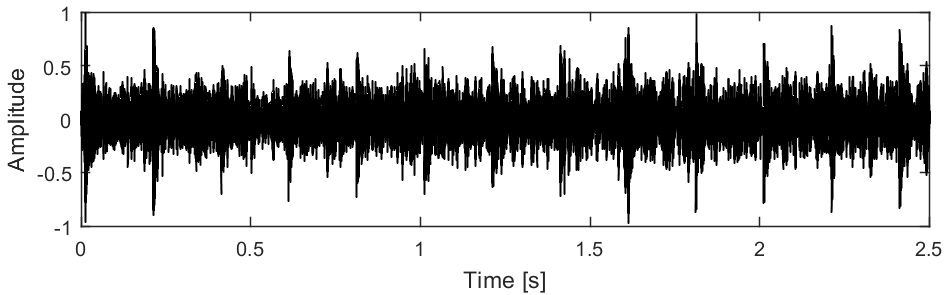
\includegraphics[width=\textwidth]{wykresy/chapter_application/semi_blind/sygnal_ff5_simulated.png}
        % \label{fig:chapter7/semi_blind/time_sim_skladowa5}
    \end{subfigure}
    %\hfill
    \begin{subfigure}[b]{0.9\textwidth}
        \centering
        \captionsetup{skip=0.01pt}
         \caption{}
        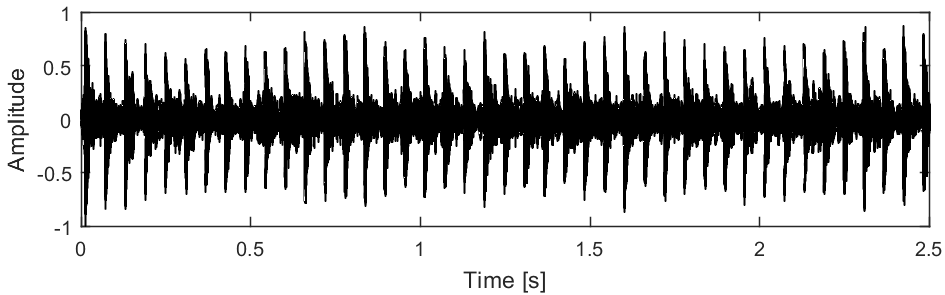
\includegraphics[width=\textwidth]{wykresy/chapter_application/semi_blind/sygnal_ff17_simulated.png}
        % \label{fig:chapter7/semi_blind/time_sim_skladowa17}
    \end{subfigure}
    \caption{Time plots of the normalized impulse trains with modulation frequencies 5~Hz (a) and 17~Hz (b).}
    \label{fig:chapter7/semi_blind/sim_skladowe}
\end{figure}
%
\begin{figure}[!ht]
    \centering
    \begin{subfigure}[b]{0.49\textwidth}
        \centering
        \captionsetup{skip=0.01pt}
        \caption{}
        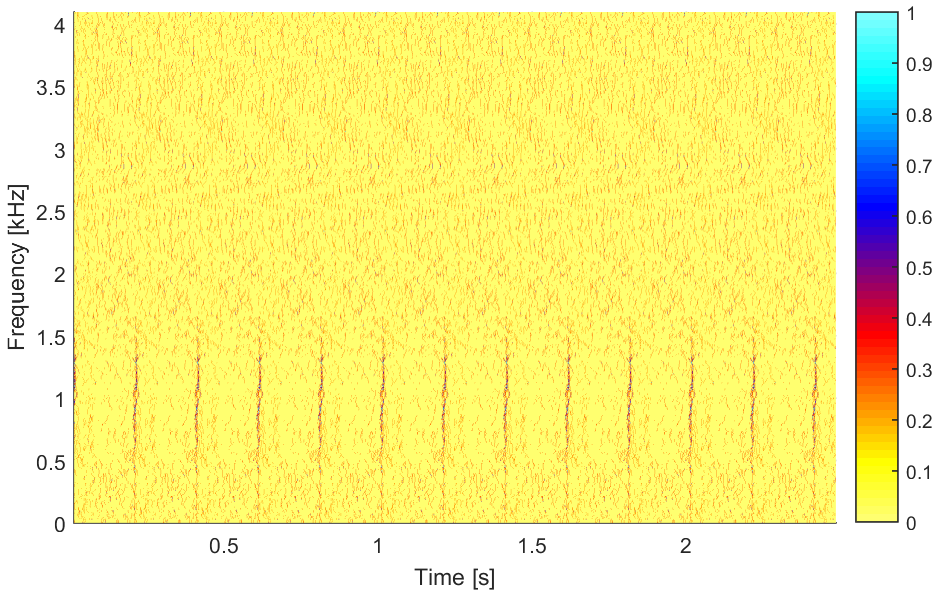
\includegraphics[width=\textwidth]{wykresy/chapter_application/semi_blind/wagi_simulated_5.png}
        \label{fig:chapter7/semi_blind/wagi_sim_5}
    \end{subfigure}
\vspace{-1\baselineskip}
    \begin{subfigure}[b]{0.49\textwidth}
        \centering
        \captionsetup{skip=0.01pt}
        \caption{}
        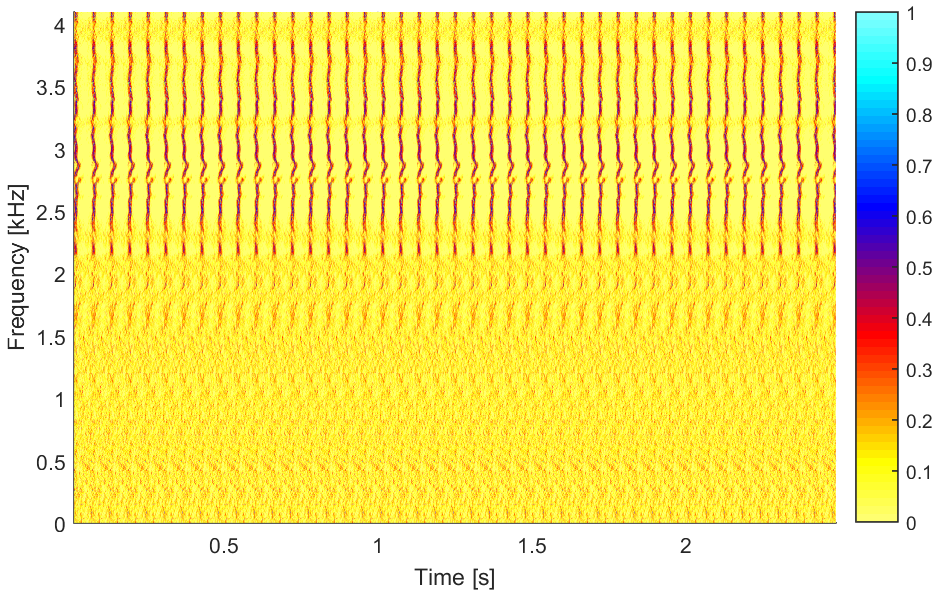
\includegraphics[width=\textwidth]{wykresy/chapter_application/semi_blind/wagi_simulated_17.png}
        \label{fig:chapter7/semi_blind/wagi_sim_17}
    \end{subfigure}
\vspace{-1\baselineskip} 
    \begin{subfigure}[b]{0.49\textwidth}
        \centering
        \captionsetup{skip=0.01pt}
        \caption{}
        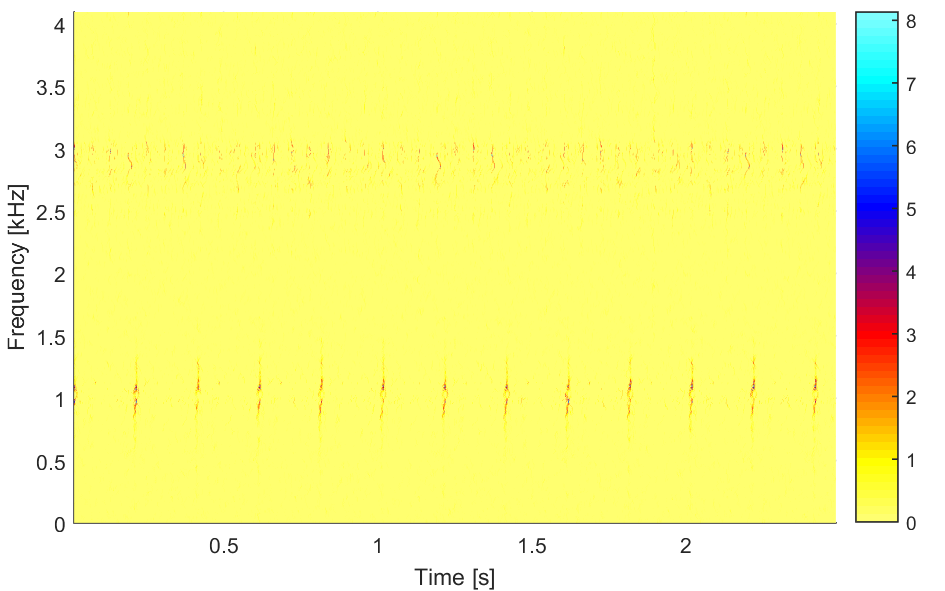
\includegraphics[width=\textwidth]{wykresy/chapter_application/semi_blind/mapka_simulated_5.png}
        \label{fig:chapter7/semi_blind/mapka_sim_5}
    \end{subfigure}
    %\hfill
    \begin{subfigure}[b]{0.49\textwidth}
        \centering
        \captionsetup{skip=0.01pt}
        \caption{}
        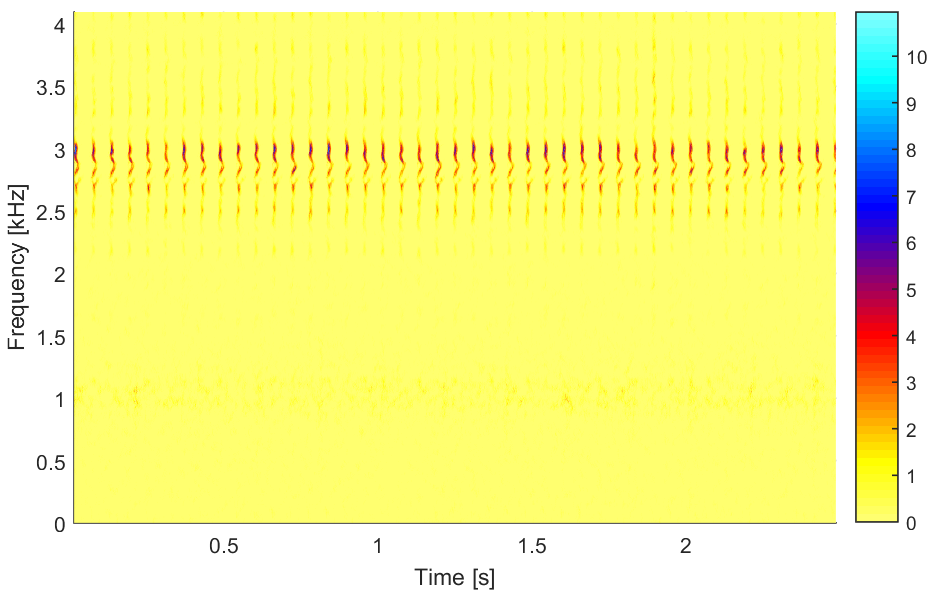
\includegraphics[width=\textwidth]{wykresy/chapter_application/semi_blind/mapka_simulated_17.png}
        \label{fig:chapter7/semi_blind/mapka_sim_17}
    \end{subfigure}
    \vspace{\baselineskip}
    \caption{Score matrices for fault frequency 5~Hz (a) and fault frequency 17~Hz (b). The weighted spectrogram (time-varying filter coefficients) for fault frequency 5~Hz (c) and fault frequency 17~Hz (d). }
    \label{fig:chapter7/semi_blind/score_sim}
\end{figure} \\
In this study we applied the proposed source separation algorithm for two different fault frequencies in order to illustrate its basic properties. Due to spectrogram parameters, the range $r$ corresponding to fault frequency 5~Hz is equal to 164. Binary maps $M$ for both cyclic frequencies are calculated and score maps are derived upon them. The score maps are presented in Figs.~\ref{fig:chapter7/semi_blind/wagi_sim_5} and~\ref{fig:chapter7/semi_blind/wagi_sim_17}. One can notice some noise in these maps, i.e. above 1500~Hz and below 2000~Hz for 5~Hz and 17~Hz cyclic frequencies, respectively. This noise is not related to the periodic amplitude modulation, since there are no clearly visible lines along the frequency axis in these frequency bands. Time-varying filter coefficients are represented by two-dimensional maps in Figs.~\ref{fig:chapter7/semi_blind/mapka_sim_5} and~\ref{fig:chapter7/semi_blind/mapka_sim_17}. Recall that these are raw spectrograms multiplied element-wise by score maps. One can notice that the random noise in score maps does not influence the filter characteristics. Non-zero scores not related to periodic modulations result in low filter coefficient, while multiplied by the spectrogram value. On the other hand, high values of the score map are related to periodic modulation and multiplication by the spectrogram values results in a high value of the time-varying filter coefficients. According to the results, the novel algorithm automatically indicates points in the spectrograms related to given fault frequencies.\\
Given two weighted spectrograms the inverse short-time Fourier transform might be applied in order to return to the time domain. In case of the simulated signal, there is a possibility to compare the raw components and the extracted time series representing sources. The comparison is presented in Fig.~\ref{fig:chapter7/semi_blind/comp_comparison_sim}. Clearly, the extracted signal components are similar to simulated. The impulses reveal in the same time points, with similar amplitudes of corresponding impulses. Moreover, the noise level is lower for extracted components, thus the impulses are even more visible. Noise level in Fig.~\ref{fig:chapter7/semi_blind/syg_comp5_sim} is about 0.3 while in the extracted signal it is close to 0.2. In case of 17~Hz amplitude modulation the noise level is close to 0.2 and 0.1 for raw and extracted signal, respectively. Presented results for the simulated data sample confirm that the proposed methodology can be applied for cyclic source extraction from the raw signal that consists of two pulse trains, each with different carrier and cyclic frequencies. In Fig.~\ref{fig:chapter7/semi_blind/widmo_comp_comparison_sim} the envelope spectra for each analyzed signal component and the corresponding extracted source signals are provided. One can observe that in both cases several harmonics related to fault frequencies are indicated. This confirms that the extracted signals follow the cyclic modulation from the raw signals. It is wort mentioning that in the raw signals only the harmonics corresponding to cyclic frequency 17~Hz were detected. (Fig.~\ref{fig:chapter7/semi_blind/obwiednia_sim}).
\begin{figure}[!ht]
    \centering
    \begin{subfigure}[b]{0.49\textwidth}
        \centering
        \captionsetup{skip=0.01pt}
        \caption{}
        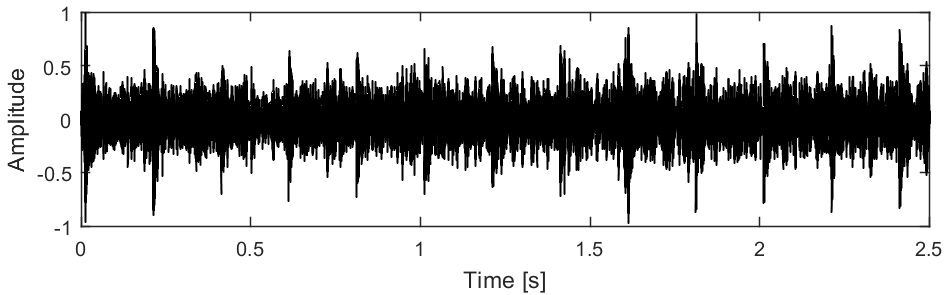
\includegraphics[width=\textwidth]{wykresy/chapter_application/semi_blind/sygnal_ff5_simulated.png}
        \label{fig:chapter7/semi_blind/syg_comp5_sim}
    \end{subfigure}
    \vspace{-1\baselineskip}
    \begin{subfigure}[b]{0.49\textwidth}
        \centering
        \captionsetup{skip=0.01pt}
        \caption{}
        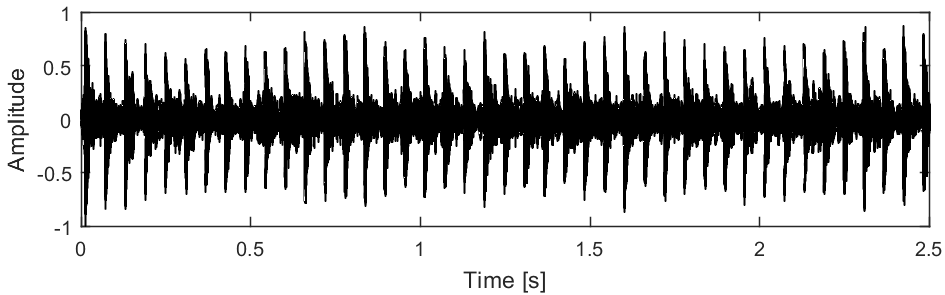
\includegraphics[width=\textwidth]{wykresy/chapter_application/semi_blind/sygnal_ff17_simulated.png}
        \label{fig:chapter7/semi_blind/syg_comp17_sim}
    \end{subfigure}
    \vspace{-1\baselineskip}  
    \begin{subfigure}[b]{0.49\textwidth}
        \centering
        \captionsetup{skip=0.01pt}
        \caption{}
        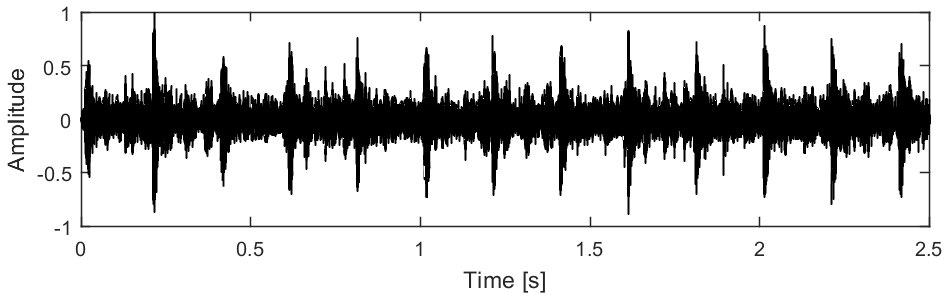
\includegraphics[width=\textwidth]{wykresy/chapter_application/semi_blind/sygnal_simulated_5.png}
        \label{fig:chapter7/semi_blind/ext_comp5_sim}
    \end{subfigure}
    %\hfill
    \begin{subfigure}[b]{0.49\textwidth}
        \centering
        \captionsetup{skip=0.01pt}
        \caption{}
        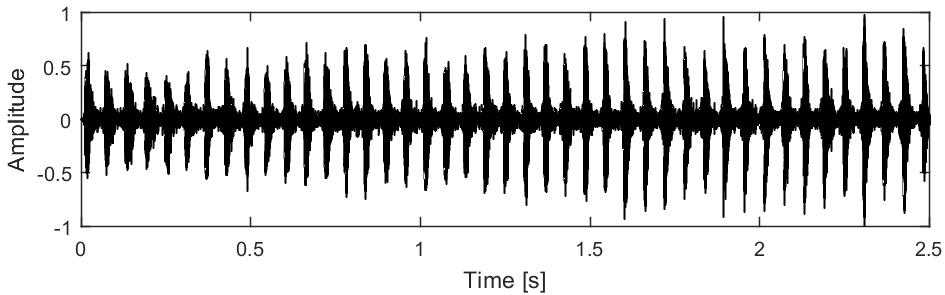
\includegraphics[width=\textwidth]{wykresy/chapter_application/semi_blind/sygnal_simulated_17.png}
        \label{fig:chapter7/semi_blind/ext_comp17_sim}
    \end{subfigure}
    \vspace{\baselineskip}
    \caption{The normalized components of the simulated signal with modulation frequency 5~Hz (a) and 17~Hz (b). The normalized extracted signal from weighted spectrogram for fault frequency 5~Hz (c) and 17~Hz(d). }
    \label{fig:chapter7/semi_blind/comp_comparison_sim}
\end{figure}
%
\begin{figure}[!ht]
    \centering
    \begin{subfigure}[b]{0.49\textwidth}
        \centering
        \captionsetup{skip=0.01pt}
        \caption{}
        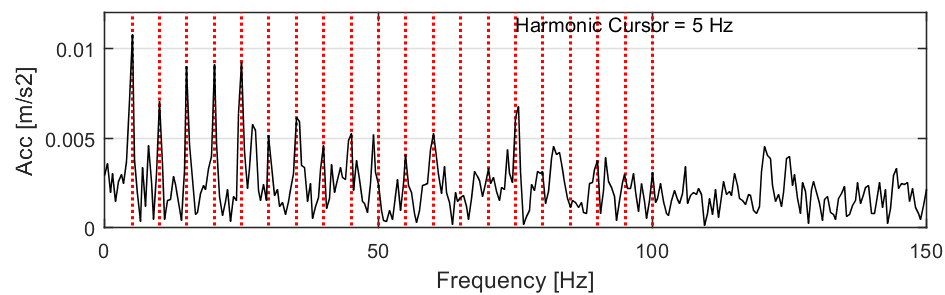
\includegraphics[width=\textwidth]{wykresy/chapter_application/semi_blind/widmo_obwiedni_simulated_comp5.png}
    \end{subfigure}
    % \vspace{-1\baselineskip}
    \begin{subfigure}[b]{0.49\textwidth}
        \centering
        \captionsetup{skip=0.01pt}
        \caption{}
    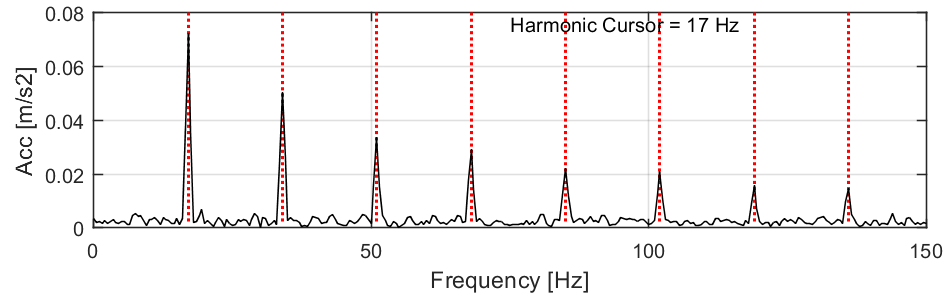
\includegraphics[width=\textwidth]{wykresy/chapter_application/semi_blind/widmo_obwiedni_simulated_comp17.png}
    \end{subfigure}
    % \vspace{-1\baselineskip}  
    \begin{subfigure}[b]{0.49\textwidth}
        \centering
        \captionsetup{skip=0.01pt}
        \caption{}
        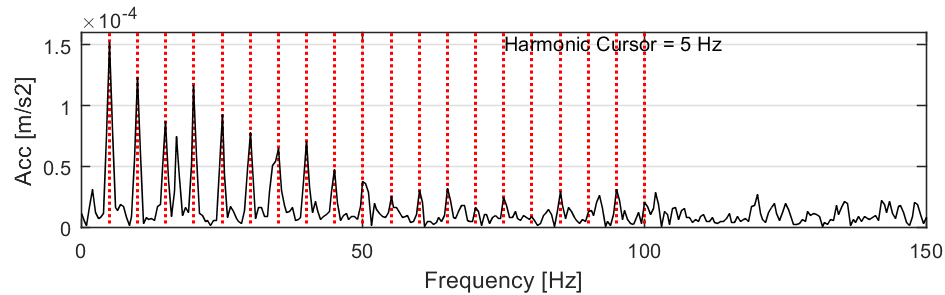
\includegraphics[width=\textwidth]{wykresy/chapter_application/semi_blind/widmo_obwiedni_simulated_5.png}
    \end{subfigure}
    %\hfill
    \begin{subfigure}[b]{0.49\textwidth}
        \centering
        \captionsetup{skip=0.01pt}
        \caption{}
        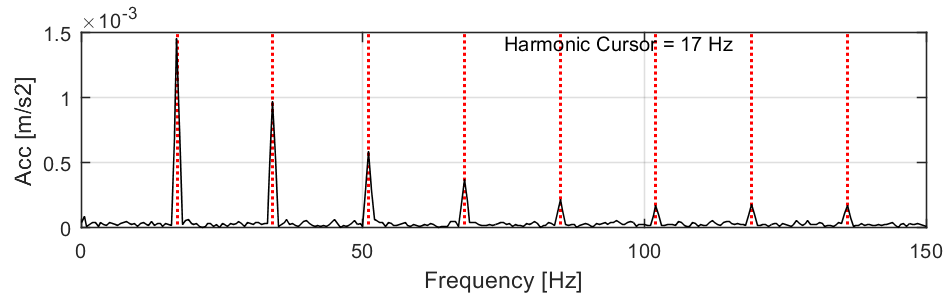
\includegraphics[width=\textwidth]{wykresy/chapter_application/semi_blind/widmo_obwiedni_simulated_17.png}
        
    \end{subfigure}
    \vspace{\baselineskip}
    \caption{The envelope spectrum of the simulated signal with modulation frequency 5~Hz (a) and 17~Hz (b). The extracted signal envelope spectrum from weighted spectrogram for fault frequency 5~Hz (c) and 17~Hz(d). }
    \label{fig:chapter7/semi_blind/widmo_comp_comparison_sim}
\end{figure}
\subsection{Signal representing bearing jitter effect}
One can be interested how the proposed method is performing in case of small variation of fault frequency. In particular, we would like to analyze the signal in which the period of the fault occurrence is not constant. Therefore, the signal, which resemble the bearing with jitter is simulated. The rotational speed is equal to 1.3 Hz and the sampling frequency is 8192~Hz. One cyclic pulse train with modulation frequency 5~Hz is added and it has a jitter effect. The carrier frequency bands are 700-1300~Hz. The amplitude of the impulses are around 1. Furthermore, the Gaussian random noise with mean 0 and standard deviation $4/3$. The waveform of the signal is presented in Fig. \ref{fig:chapter7/semi_blind/time_jitter}. 
\begin{figure}[!ht]
    \centering
    \begin{subfigure}[b]{0.8\textwidth}
        \centering
        \captionsetup{skip=0.01pt}
         \caption{}
        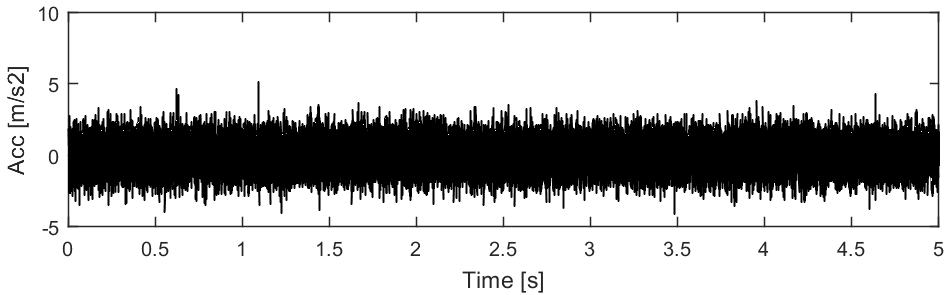
\includegraphics[width=\textwidth]{wykresy/chapter_application/semi_blind/sygnal_jitter.png}
        \label{fig:chapter7/semi_blind/time_jitter}
    \end{subfigure}
    %\hfill
    \begin{subfigure}[b]{0.7\textwidth}
        \centering
        \captionsetup{skip=0.01pt}
         \caption{}
        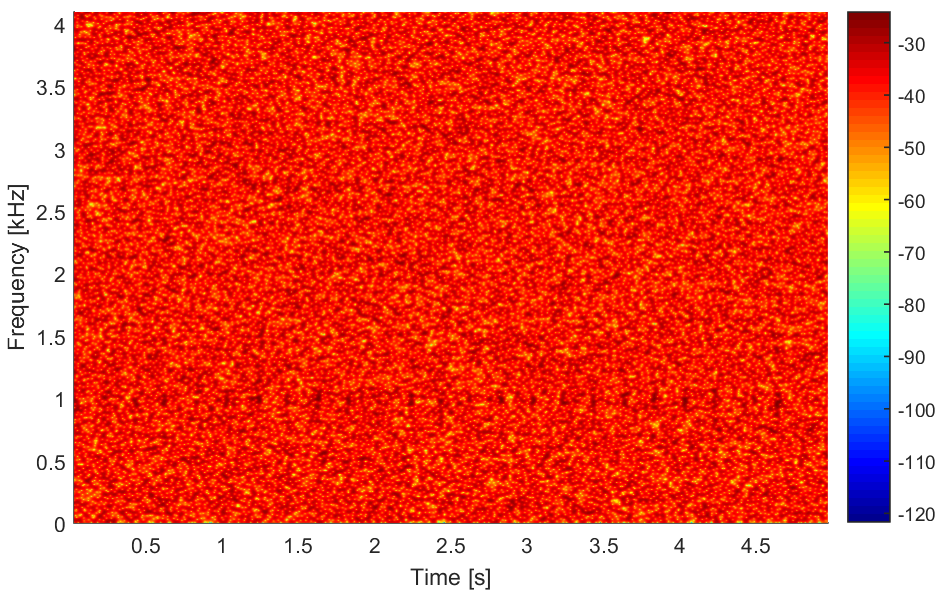
\includegraphics[width=\textwidth]{wykresy/chapter_application/semi_blind/spectrogram_jitter.png}
        \label{fig:chapter7/semi_blind/spectrogram_jitter}
    \end{subfigure}
%    \hfill
    \begin{subfigure}[b]{0.8\textwidth}
        \centering
        \captionsetup{skip=0.01pt}
        \caption{}
        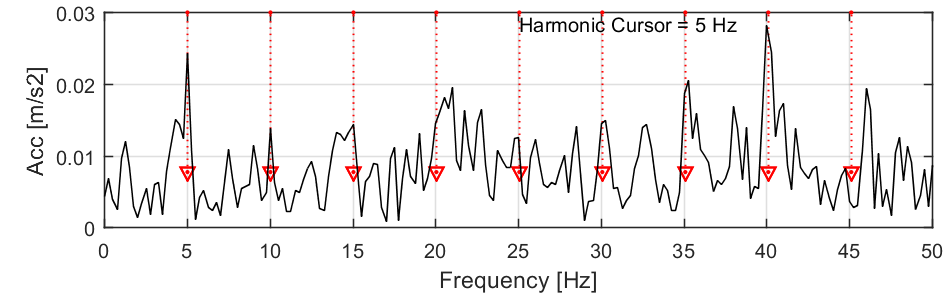
\includegraphics[width=\textwidth]{wykresy/chapter_application/semi_blind/widmo_obwiedni_jitter.png}
        \label{fig:chapter7/semi_blind/obwiednia_jitter}
    \end{subfigure}
    \caption{Time plot (a), spectrogram (b) and envelope spectrum (c) of the vibration simulated signal with bearing jitter effect. The spectrogram parameters are as follows: $N_w=250$, $Ov=96\%$.}
\end{figure}
The impulses are barely visible on the time-frequency map (Fig. \ref{fig:chapter7/semi_blind/spectrogram_jitter}). Furthermore, on the envelope spectrum the harmonics correspond to fault frequency cannot be observed (Fig. \ref{fig:chapter7/semi_blind/obwiednia_jitter}). Thus, it is a complicated signal with invisible fault component, where the standard envelope methods for fault detection fail. Therefore, we would like to apply proposed method for cyclic source extraction. The extracted cyclic normalized signal component is presented in Fig. \ref{fig:chapter7/semi_blind/time_jitter_filtr}. One can observe that the level of noise is smaller and the impulses are clearly detectable. As it was expected on the envelope spectrum the harmonics related to the fault frequency are observed, namely 7 harmonics are visible. It is shown that the proposed algorithm is performing well in case of the signal with slightly varying fault frequency. Obviously, the results depend on the level of fault frequency variances. However, in case of the reasonable changes of the period of fault occurrence the method is able to extract the signal component related to the fault.
%
\begin{figure}[!ht]
    \centering
    \begin{subfigure}[b]{0.8\textwidth}
        \centering
        \captionsetup{skip=0.01pt}
         \caption{}
        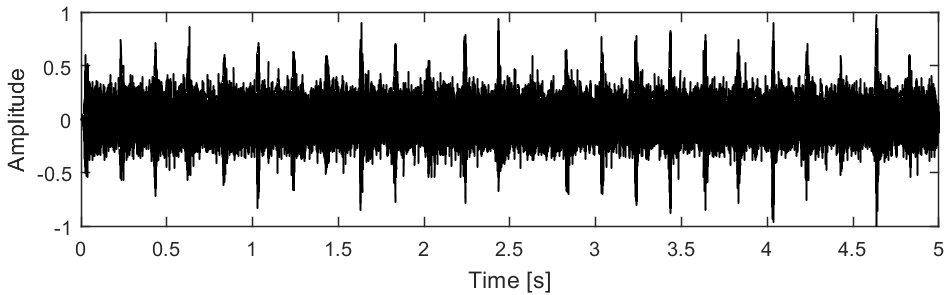
\includegraphics[width=\textwidth]{wykresy/chapter_application/semi_blind/sygnal_jitter_filtr.png}
        \label{fig:chapter7/semi_blind/time_jitter_filtr}
    \end{subfigure}

    \begin{subfigure}[b]{0.8\textwidth}
        \centering
        \captionsetup{skip=0.01pt}
        \caption{}
        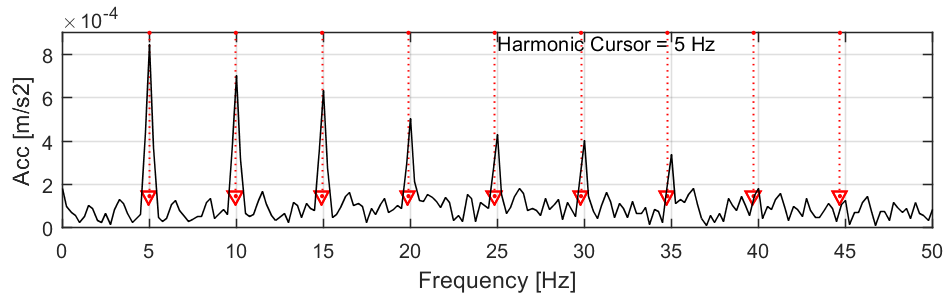
\includegraphics[width=\textwidth]{wykresy/chapter_application/semi_blind/widmo_obwiedni_jitter_filtr.png}
        \label{fig:chapter7/semi_blind/obwiednia_jitter_filtr}
    \end{subfigure}
    \caption{Time plot (a) and envelope spectrum (b) of the extracted cyclic normalized signal component with bearing jitter effect.}
\end{figure}
%
\subsection{Signal without cyclic component}
Finally, we would like to test the performance of the method for the healthy signal. Indeed, the signal without any cyclic component is simulated. The length is equal to 2.5 seconds and the sampling frequency is 8192~Hz. The signal consists of background Gaussian random noise with mean zero and variance equal to 0.2. Furthermore, in the carrier frequency bands 700-1300~Hz and 2300-3200~Hz additional random noise with mean zero and variance  0.2 is added. Therefore, it is signal like in section \ref{sec:chapter7/semi_blind/schemat_przekladniamultiple source} with amplitude of impulses equals to 0. In the analysis the proposed cyclic source extraction method was tested for the modulation frequency 17~Hz. It is expected that as a result, the signal without fault pattern is obtained. It would ensure that the proposed method do not create the cyclic impulses. In Fig. \ref{fig:chapter7/semi_blind/time_zdrowy} the signal without cyclic component is presented. Furthermore, the spectrogram is shown in Fig. \ref{fig:chapter7/semi_blind/spectrogram_zdrowy}, where no impulses are visible. In the envelope spectrum no harmonics of modulation frequency 17~Hz are observed. 
\begin{figure}[!ht]
    \centering
    \begin{subfigure}[b]{0.8\textwidth}
        \centering
        \captionsetup{skip=0.01pt}
         \caption{}
        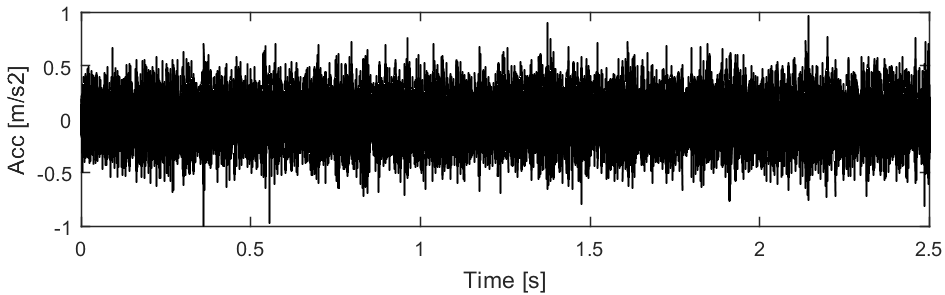
\includegraphics[width=\textwidth]{wykresy/chapter_application/semi_blind/sygnal_bez_impulsow.png}
        \label{fig:chapter7/semi_blind/time_zdrowy}
    \end{subfigure}
    %\hfill
    \begin{subfigure}[b]{0.7\textwidth}
        \centering
        \captionsetup{skip=0.01pt}
         \caption{}
        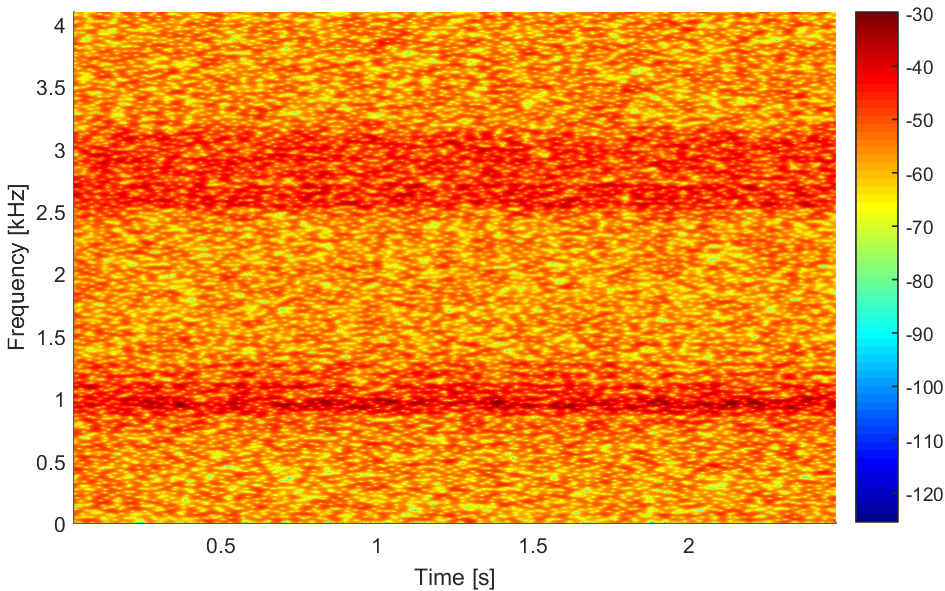
\includegraphics[width=\textwidth]{wykresy/chapter_application/semi_blind/spectrogramsygnal_bez_impulsow.png}
        \label{fig:chapter7/semi_blind/spectrogram_zdrowy}
    \end{subfigure}
%    \hfill
    \begin{subfigure}[b]{0.8\textwidth}
        \centering
        \captionsetup{skip=0.01pt}
        \caption{}
        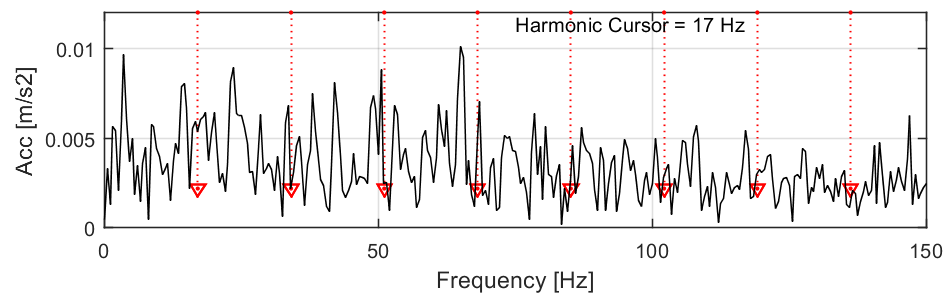
\includegraphics[width=\textwidth]{wykresy/chapter_application/semi_blind/widmo_obwiedni_sygnal_bez_impulsow.png}
        \label{fig:chapter7/semi_blind/obwiednia_zdrowy}
    \end{subfigure}
    \caption{Time plot (a), spectrogram (b) and envelope spectrum (c) of the vibration simulated signal without the fault component. The spectrogram parameters are as follows: $N_w=250$, $Ov=96\%$.}
    \end{figure}
%
The signal after source extraction method application is presented in Fig. \ref{fig:chapter7/semi_blind/time_zdrowy_filtr}. One can observe that it is similar to signal before the processing (Fig. \ref{fig:chapter7/semi_blind/obwiednia_zdrowy}). In the envelope spectrum the harmonics related to the modulation frequency 17~Hz are not observed (Fig. \ref{fig:chapter7/semi_blind/obwiednia_zdrowy_filtr}). Therefore, the proposed method do not create the false alarms. It means that it can be applied to the machine without the local fault and the extracted signal would not contain the cyclic impulses. Presented analysis on the simulated signal ensure that the method is powerful in case of detection the cyclic impulses. 
\begin{figure}
    \centering
    \begin{subfigure}[b]{0.8\textwidth}
        \centering
        \captionsetup{skip=0.01pt}
         \caption{}
        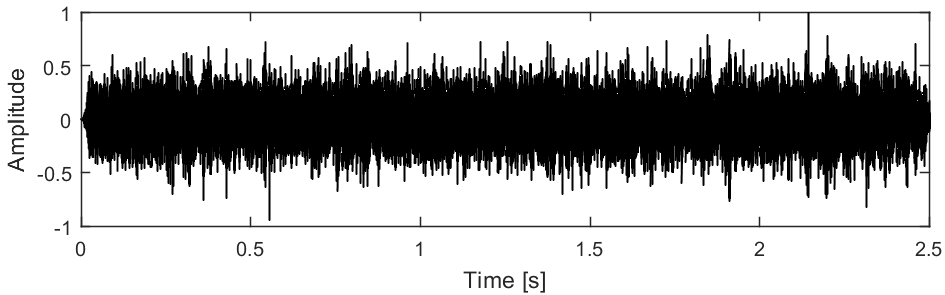
\includegraphics[width=\textwidth]{wykresy/chapter_application/semi_blind/sygnal_bez_impulsow_filtr.png}
        \label{fig:chapter7/semi_blind/time_zdrowy_filtr}
    \end{subfigure}

    \begin{subfigure}[b]{0.8\textwidth}
        \centering
        \captionsetup{skip=0.01pt}
        \caption{}
        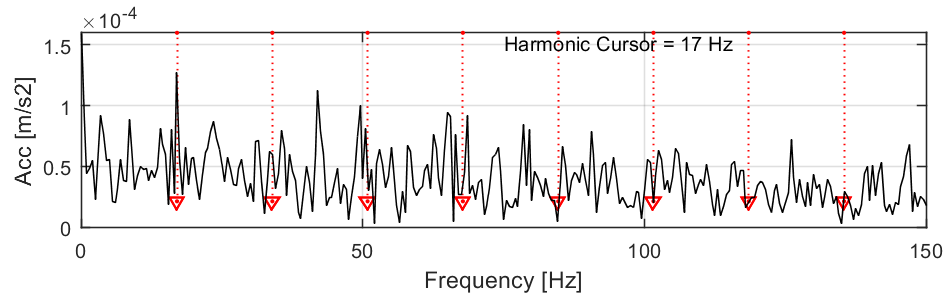
\includegraphics[width=\textwidth]{wykresy/chapter_application/semi_blind/widmo_obwiedni_sygnal_bez_impulsow_filtr.png}
        \label{fig:chapter7/semi_blind/obwiednia_zdrowy_filtr}
    \end{subfigure}
    \caption{Time plot (a) and envelope spectrum (b) of the extracted cyclic normalized signal component with bearing jitter effect.}
\end{figure}
\section{Real data analysis}
\subsection{Cyclic sources extraction from complex multiple-component vibration signal via periodically time varying filter}
\label{sec:chapter7/semi_blind/schemat_przekladniaapplication_real}
Once the performance of the algorithm was tested on the simulated data, it can be applied to the real signal. In this section results of the methodology application to the vibration data recorded on the belt conveyor gearbox are presented. Analyzed machine is located in the underground copper ore mine, thus it works in harsh environment. Kinematic scheme of the analyzed gearbox is presented in Fig.~\ref{fig:chapter7/semi_blind/schemat_przekladnia}. The gearbox is equipped with two stages - the first bevel pair is followed by the spur pair. The electric engine rotor speed is around 996 rpm, thus the first shaft rotates with the frequency close to 16.61~Hz. Variability of the rotational speed does not exceed $\pm1.5$ rpm. The rotational frequency of the second shaft is 4.2~Hz, since the first stage ratio is equal to 91:23. The vibration signal was acquired on three different spots of the machine (Fig.~\ref{fig:chapter7/semi_blind/pomiar}). Moreover, the rotational speed was also acquired in order to ensure that it is almost constant during the experiment. Sampling frequency is 17066~Hz and the signal duration is equal to 5 seconds. The exemplary local fault in the gear is illustrated in Fig.~\ref{fig:chapter7/semi_blind/damage}.
%
\begin{figure}[ht!]
\centering
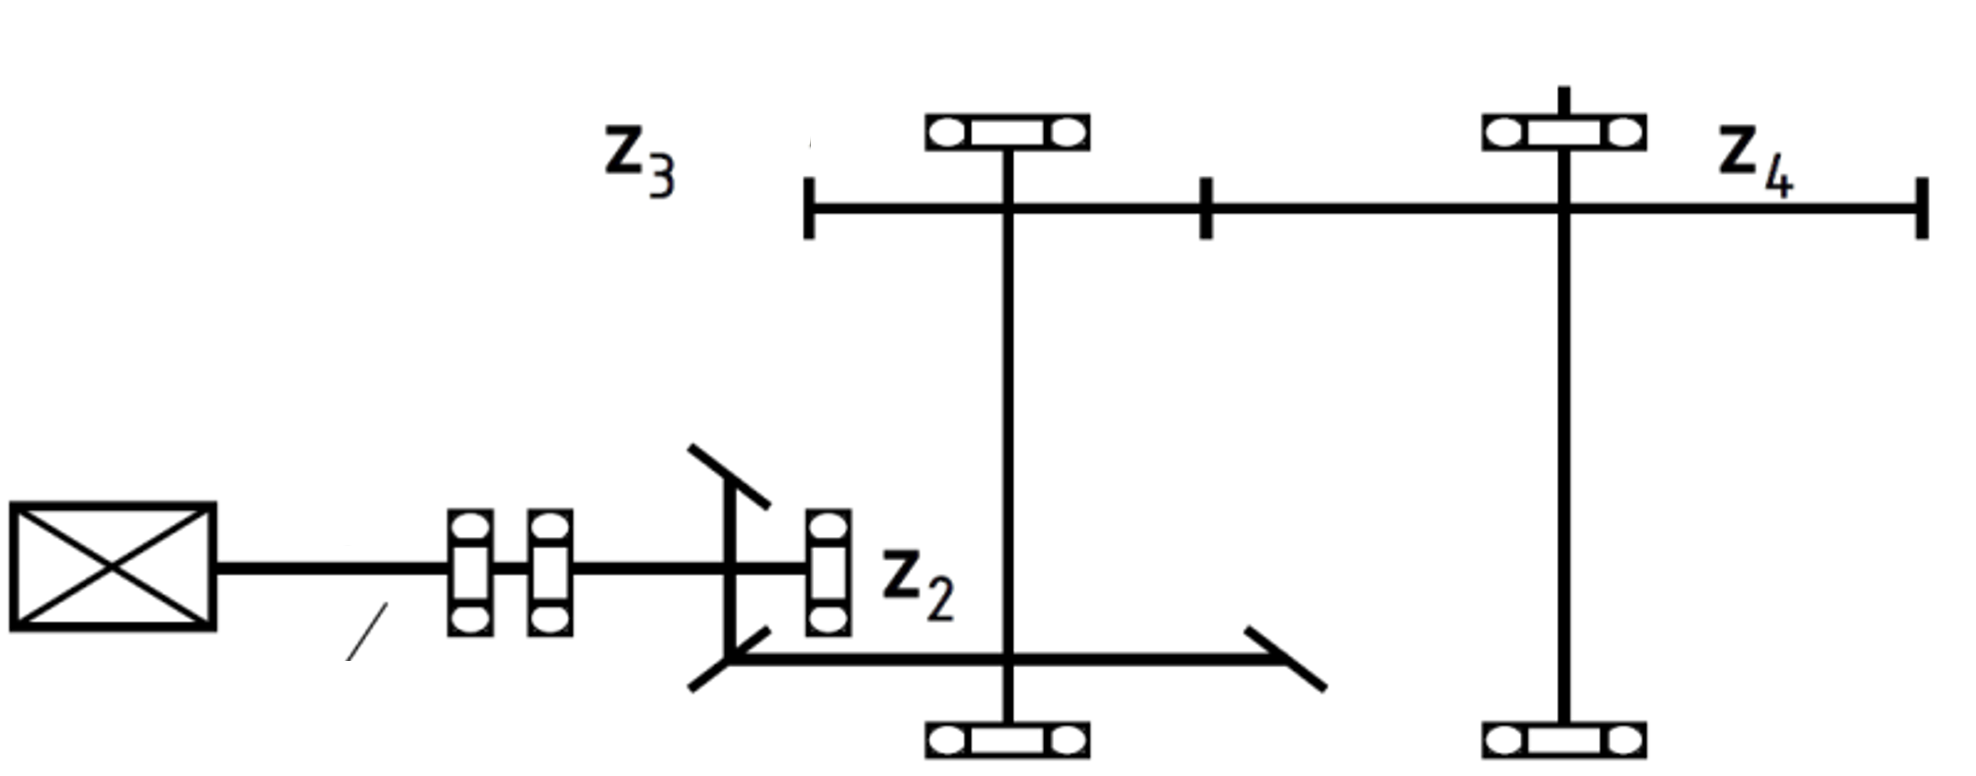
\includegraphics[width=1\textwidth]{wykresy/chapter_application/semi_blind/schemat_przekladnia}
\caption{Kinematic scheme of the analyzed gearbox. The number of teeth in each stage: $z_1=23$, $z_2=91$, $z_3=44$ and $z_4=155$.}
\label{fig:chapter7/semi_blind/schemat_przekladnia}
\end{figure}
%
\begin{figure}[!ht]
    \centering
    \begin{subfigure}[b]{0.49\textwidth}
        \centering
        \captionsetup{skip=0.01pt}
        \caption{}
        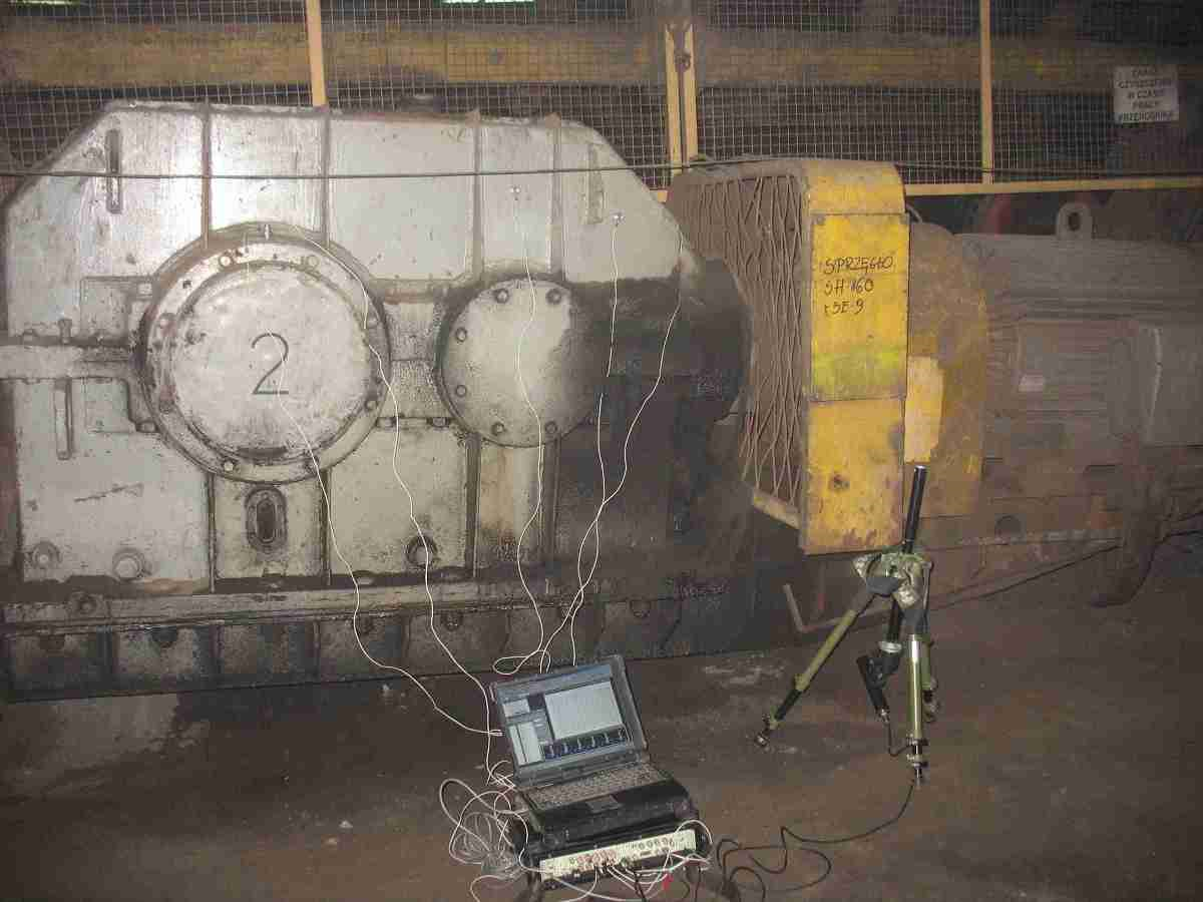
\includegraphics[width=\textwidth]{wykresy/chapter_application/semi_blind/czujniki}
        \label{fig:chapter7/semi_blind/pomiar}
    \end{subfigure}
    %\hfill
    \begin{subfigure}[b]{0.49\textwidth}
        \centering
        \captionsetup{skip=0.01pt}
        \caption{}
        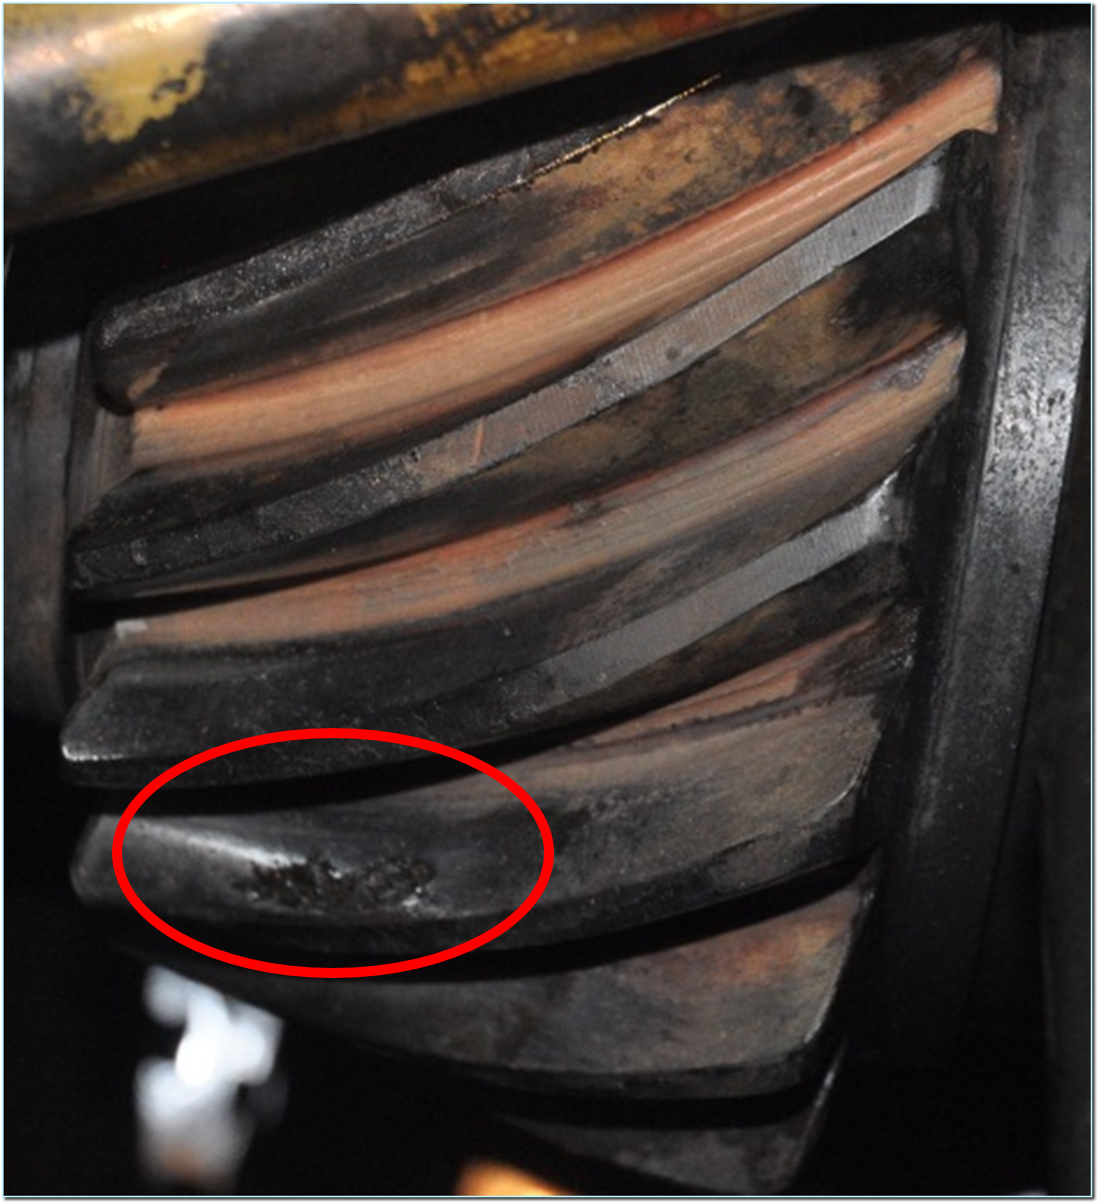
\includegraphics[width=\textwidth]{wykresy/chapter_application/semi_blind/damage}
        \label{fig:chapter7/semi_blind/damage}
    \end{subfigure}    
    \caption{The data acquisition system during the experiment (a) and exemplary local damage in the gear (b).}
\end{figure}
%
\\
The signal reveals two faults in the machine related to the rotating speed of first and second shaft. The signal in time domain is presented in Fig.~\ref{fig:chapter7/semi_blind/time_L212}. The raw spectrogram (Fig.~\ref{fig:chapter7/semi_blind/spectrogram_L212}) reveals some frequency bands with high energy. These are related to gear mesh frequencies (379.5~Hz and 183.3~Hz for first and second stage, respectively) and their harmonics. There are lots of  wideband excitations, although it is difficult to state if they are related to any cyclic pattern. Thus, it is worth to apply the proposed source extraction algorithm.
\begin{figure}
    \centering
    \vspace{-1\baselineskip}
    \begin{subfigure}[b]{0.8\textwidth}
        \centering
        \captionsetup{skip=0.01pt}
        \caption{}
        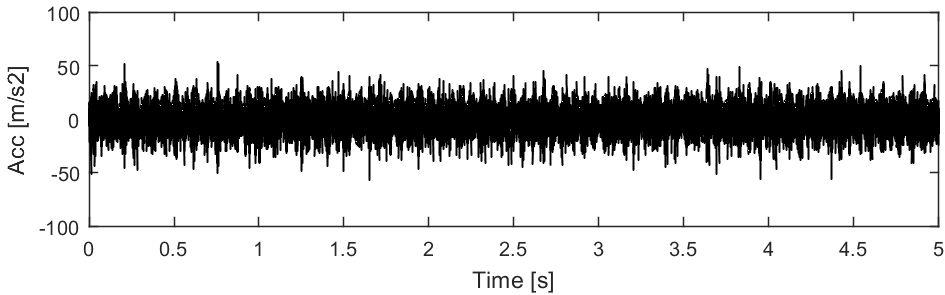
\includegraphics[width=\textwidth]{wykresy/chapter_application/semi_blind/sygnalL212.png}
        \label{fig:chapter7/semi_blind/time_L212}
    \end{subfigure}
     \vspace{-1\baselineskip}
    \begin{subfigure}[b]{0.8\textwidth}
        \centering
        \captionsetup{skip=0.01pt}
        \caption{}
        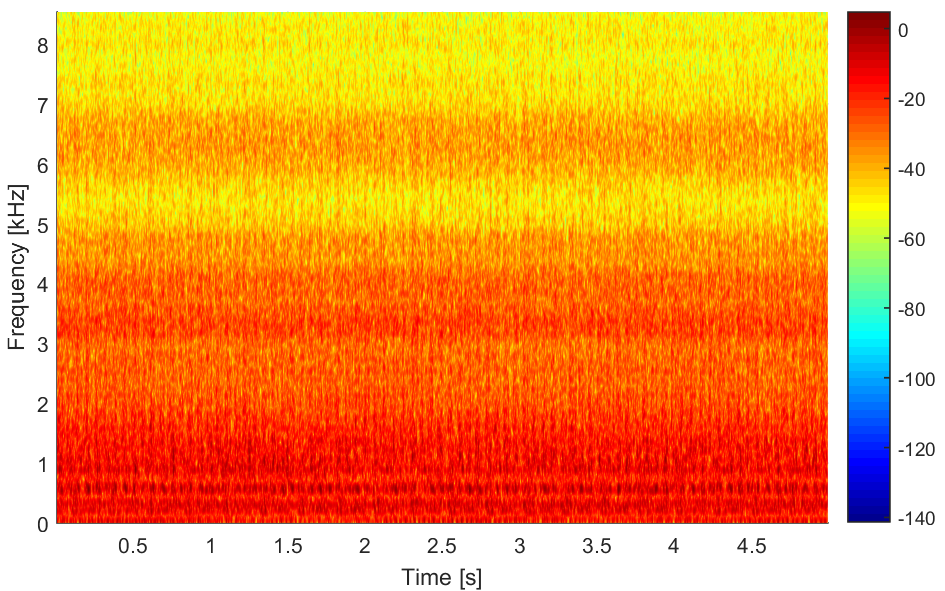
\includegraphics[width=\textwidth]{wykresy/chapter_application/semi_blind/spectrogramL212.png}
        \label{fig:chapter7/semi_blind/spectrogram_L212}
    \end{subfigure}
    \begin{subfigure}[b]{0.8\textwidth}
        \centering
        \captionsetup{skip=0.01pt}
        \caption{}
        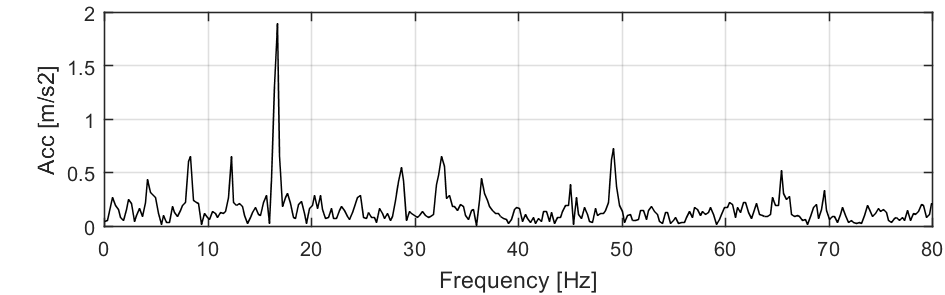
\includegraphics[width=\textwidth]{wykresy/chapter_application/semi_blind/widmo_obwiedniL212.png}
        \label{fig:chapter7/semi_blind/obwiednia_L212}
    \end{subfigure}
    \caption{Time plot (a), spectrogram (b) and envelope spectrum (c) of the real signal recorded on the belt conveyor's gearbox. The spectrogram parameters are as follows: $N_w=250$, $Ov=96\%$.}\label{fig:chapter7/semi_blind/time-plot_L212}
\end{figure}
\\
As in the simulated data case, two fault frequencies are considered, namely, 4.2~Hz and 16.61~Hz. Score maps for two fault frequencies are presented in Figs.~\ref{fig:chapter7/semi_blind/wagi_L212_4} and~\ref{fig:chapter7/semi_blind/wagi_L212_16}. Some barely visible periodic patterns might be noticed in both figures. The pattern related to 4.2~Hz is located in carrier frequency band lower than 1000~Hz. The second pattern reveals in almost every frequency band, including the lowest frequencies. Thus, this signal is more challenging than the simulated data, since in a single frequency band two periodic modulations occur and one of them reveals in a relatively narrow frequency band. Moreover, two different phases can be detected in case of 4.2~Hz modulation frequency (see arrows in Fig.~\ref{fig:chapter7/semi_blind/wagi_L212_4}), i.e. two different components with modulation frequency close to 4.2~Hz can be noticed. The related carrier frequencies are 0-400~Hz and 500-700~Hz, respectively. Such phenomenon might be caused by two different local faults occurring on the second shaft, for instance one on the bevel gear and second on the spur gear. Therefore, carrier frequency bands might be different due to different transmission path.
\begin{figure}[!ht]
    \centering
    \begin{subfigure}[b]{0.49\textwidth}
        \centering
        \captionsetup{skip=0.01pt}
        \caption{}
        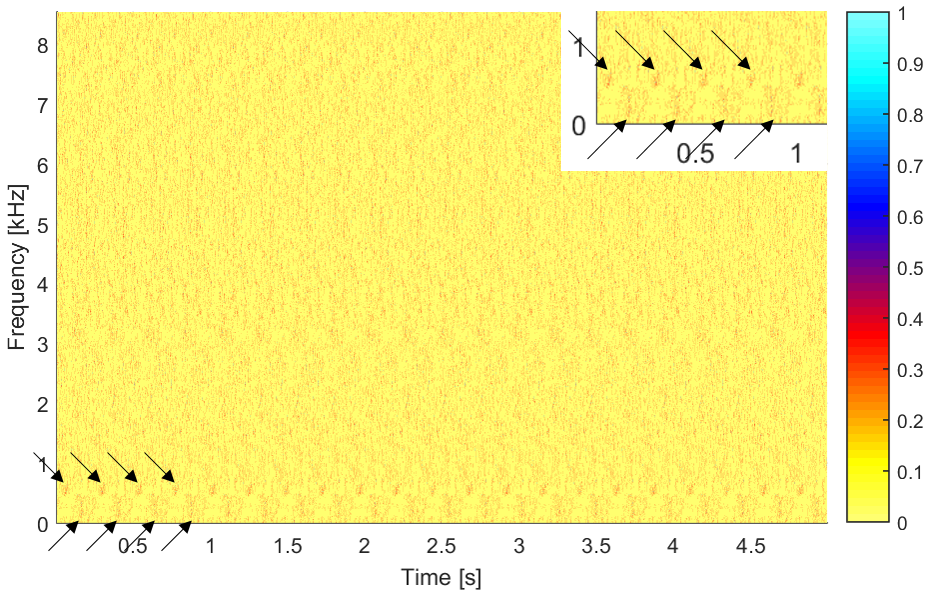
\includegraphics[width=\textwidth]{wykresy/chapter_application/semi_blind/wagiL212_4.png}
        \label{fig:chapter7/semi_blind/wagi_L212_4}
    \end{subfigure}
     \vspace{-1\baselineskip}
    \begin{subfigure}[b]{0.49\textwidth}
        \centering
        \captionsetup{skip=0.01pt}
        \caption{}
        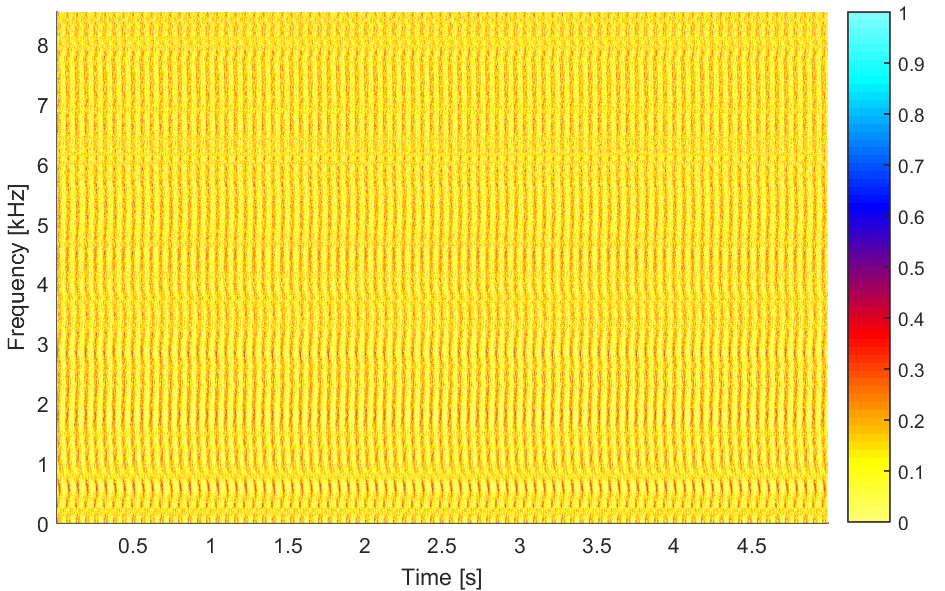
\includegraphics[width=\textwidth]{wykresy/chapter_application/semi_blind/wagiL212_16.png}
        \label{fig:chapter7/semi_blind/wagi_L212_16}
    \end{subfigure}
     \vspace{-1\baselineskip}
    \begin{subfigure}[b]{0.49\textwidth}
        \centering
        \captionsetup{skip=0.01pt}
        \caption{}
        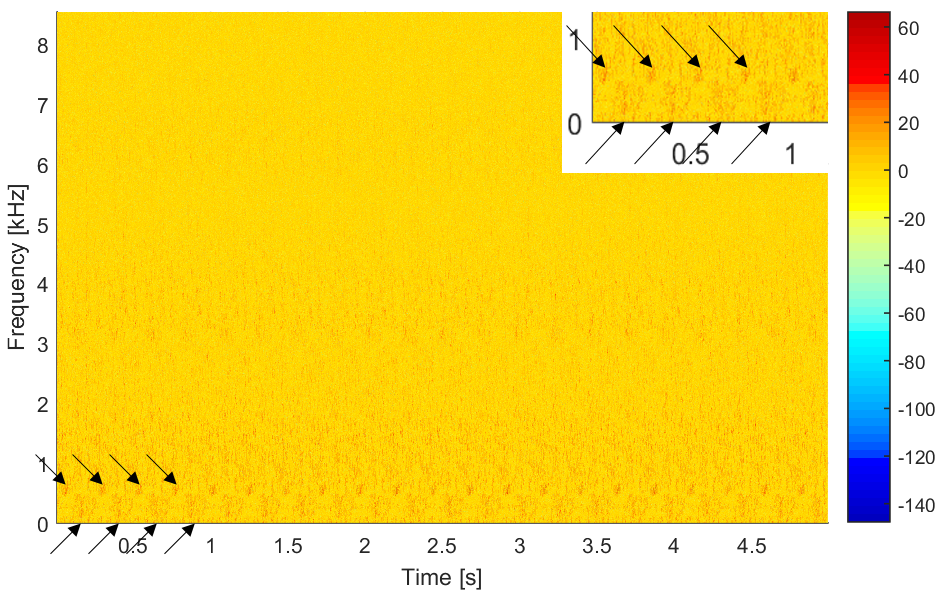
\includegraphics[width=\textwidth]{wykresy/chapter_application/semi_blind/mapkaL212_log_4.png}
        \label{fig:chapter7/semi_blind/mapka_L212_4}
    \end{subfigure}
    %\hfill
    \begin{subfigure}[b]{0.49\textwidth}
        \centering
        \captionsetup{skip=0.01pt}
        \caption{}
        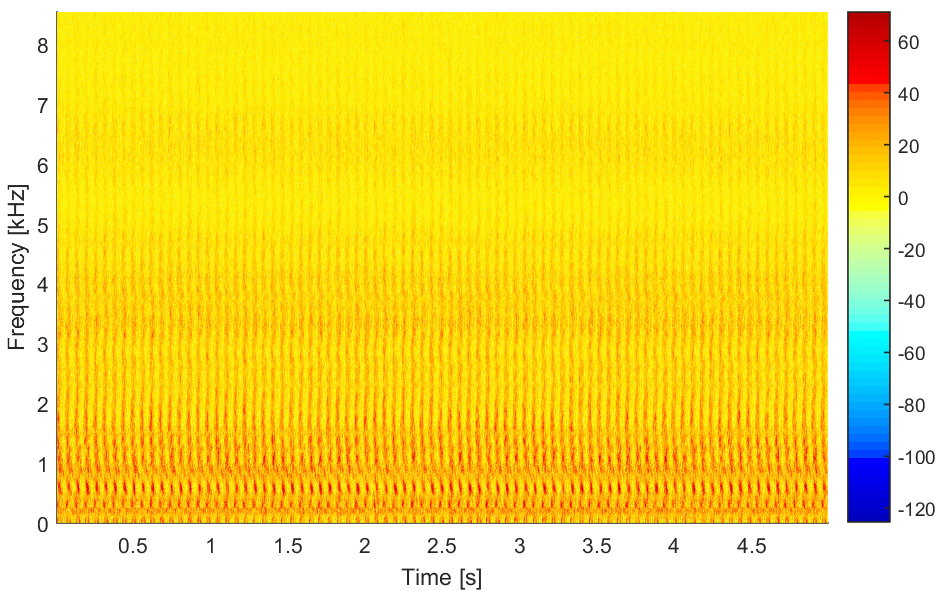
\includegraphics[width=\textwidth]{wykresy/chapter_application/semi_blind/mapkaL212_log_16.png}
        \label{fig:chapter7/semi_blind/mapka_L212_16}
    \end{subfigure}
    \caption{Score matrices for fault frequency 4.2~Hz (a) and 16.61~Hz (b). The weighted spectrograms in the log scale for fault frequency 4.2~Hz (c) and 16.61~Hz (d). }\label{fig:chapter7/semi_blind/score_real}
%
% zoomed maps
    \centering
    \begin{subfigure}[b]{0.49\textwidth}
        \centering
        \captionsetup{skip=0.01pt}
        \caption{}
        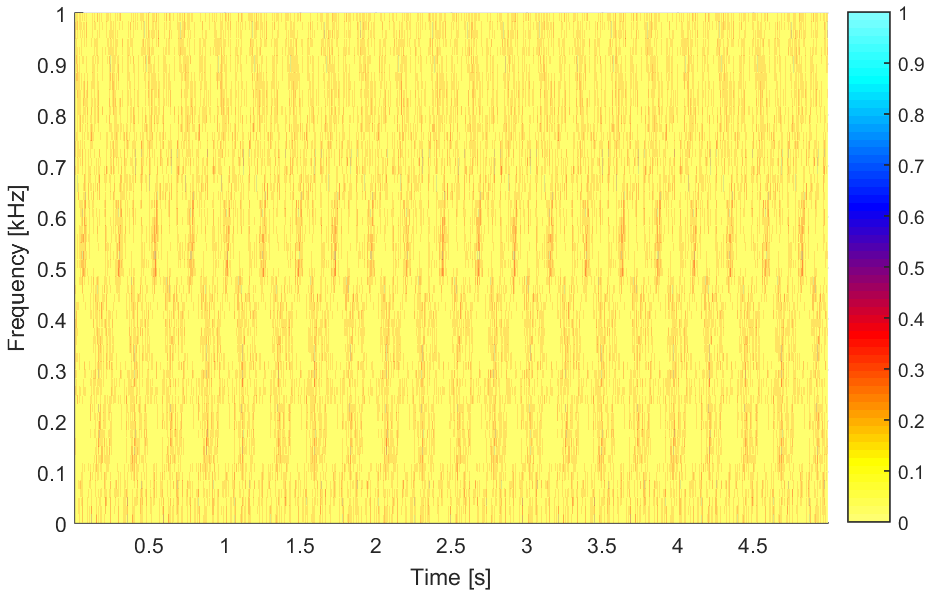
\includegraphics[width=\textwidth]{wykresy/chapter_application/semi_blind/wagiL212_4_zoom.png}
    \end{subfigure}
    %\hfill
    \begin{subfigure}[b]{0.49\textwidth}
        \centering
        \captionsetup{skip=0.01pt}
        \caption{}
        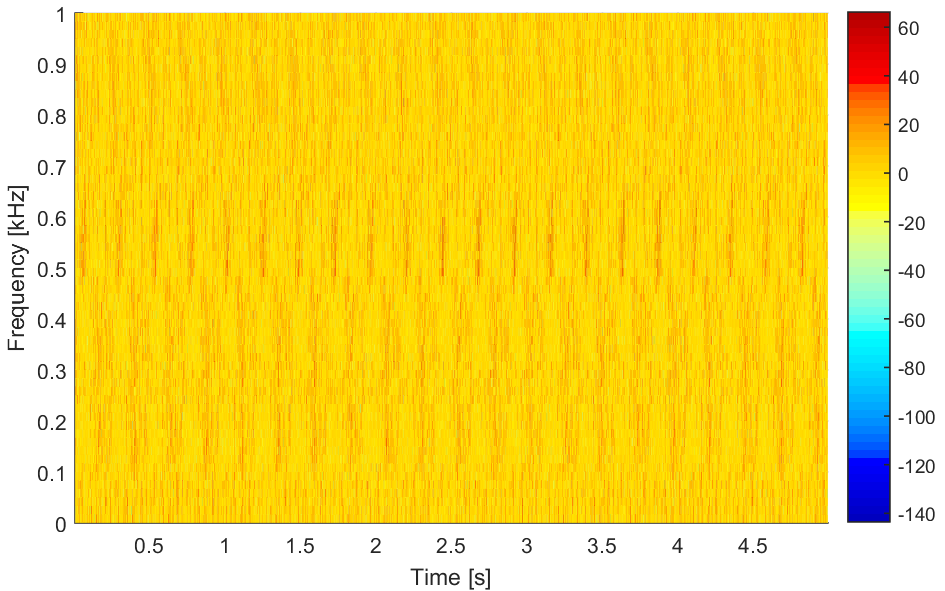
\includegraphics[width=\textwidth]{wykresy/chapter_application/semi_blind/mapkaL212_log_4_zoom.png}
    \end{subfigure}    
    \caption{The zoomed score matrix for fault frequency 4.2~Hz (a) and zoomed weighted spectrogram in the log scale for fault frequency 4.2~Hz (b).}\label{fig:chapter7/semi_blind/score_zoom}
\end{figure}
%
% widma obwiedni
\begin{figure}[!ht]
    \centering
    \begin{subfigure}[b]{0.49\textwidth}
        \centering
        \captionsetup{skip=0.01pt}
        \caption{}
        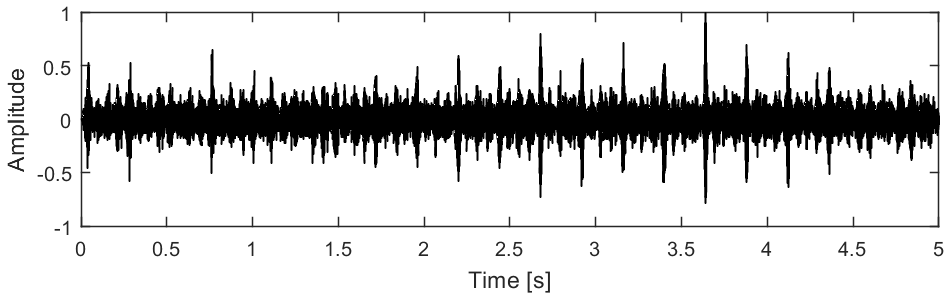
\includegraphics[width=\textwidth]{wykresy/chapter_application/semi_blind/sygnalL212_4.png}
        \label{fig:chapter7/semi_blind/ext_comp_L212_4}
    \end{subfigure}
     \vspace{-1\baselineskip}
    \begin{subfigure}[b]{0.49\textwidth}
        \centering
        \captionsetup{skip=0.01pt}
        \caption{}
        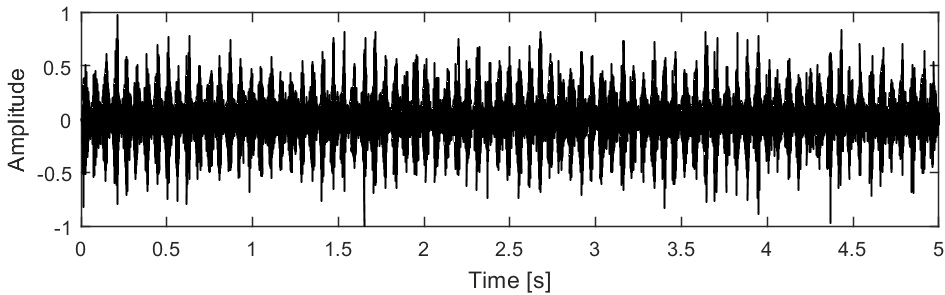
\includegraphics[width=\textwidth]{wykresy/chapter_application/semi_blind/sygnalL212_16.png}
        \label{fig:chapter7/semi_blind/ext_comp_L212_16}
    \end{subfigure}
     \vspace{-1\baselineskip}
    \begin{subfigure}[b]{0.49\textwidth}
        \centering
        \captionsetup{skip=0.01pt}
        \caption{}
        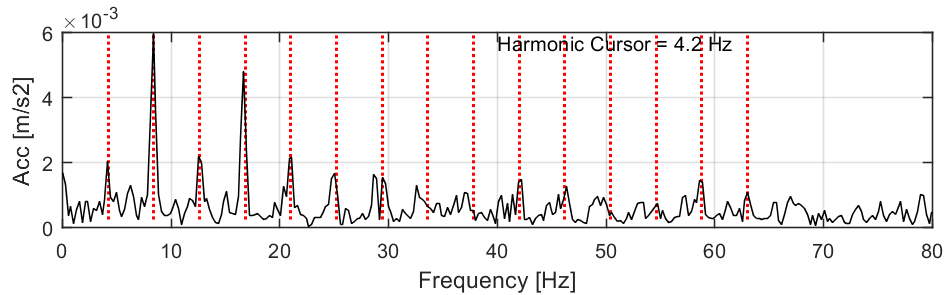
\includegraphics[width=\textwidth]{wykresy/chapter_application/semi_blind/widmo_obwiedniL212_4.png}
        \label{fig:chapter7/semi_blind/ext_widmo_obwiedni_L212_4}
    \end{subfigure}
        \begin{subfigure}[b]{0.49\textwidth}
        \centering
        \captionsetup{skip=0.01pt}
        \caption{}
        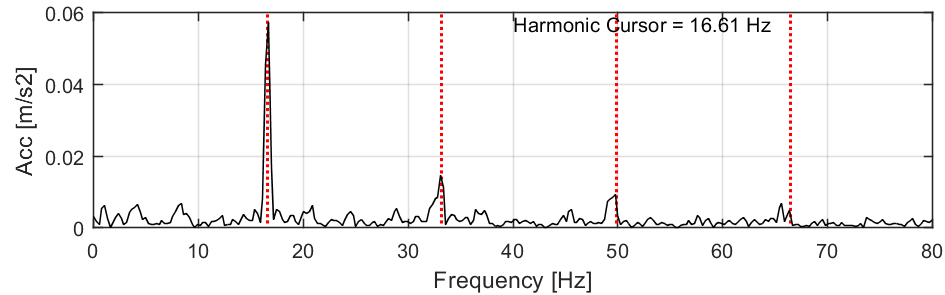
\includegraphics[width=\textwidth]{wykresy/chapter_application/semi_blind/widmo_obwiedniL212_16.png}
        \label{fig:chapter7/semi_blind/ext_widmo_obwiedni_L212_16}
    \end{subfigure}
    \vspace{\baselineskip}
    \caption{The normalized extracted signals from weighted spectrograms for fault frequency 4.2~Hz (a) and 16.61~Hz (b). The envelope spectra of the extracted signals for fault frequency 4.2~Hz (c) and 16.61~Hz (d). }\label{fig:chapter7/semi_blind/signal_ext}
\end{figure} 


Weighted spectrograms are illustrated in Figs.~\ref{fig:chapter7/semi_blind/mapka_L212_4} and~\ref{fig:chapter7/semi_blind/mapka_L212_16}. One can observe that the level of background noise is relatively small and the periodic excitations are with relatively high amplitudes.  In order to transform weighted spectrogram to time domain the inverse short-time Fourier transform can be applied. Therefore, the cyclic component is extracted. The results are presented in Figs.~\ref{fig:chapter7/semi_blind/ext_comp_L212_4} and~\ref{fig:chapter7/semi_blind/ext_comp_L212_16}. Two different in phase pulse trains with modulation frequency 4.2~Hz might not be clearly visible, since the corresponding score values are relatively low. Excitations related to the second fault are clearly visible. Given the extracted components, envelope analysis might be performed in order to check periodicity of the extracted signals. According to Figs.~\ref{fig:chapter7/semi_blind/ext_widmo_obwiedni_L212_4} more than 10 harmonics of 4.2~Hz might be noticed which corresponds to impulsive character of the source signal. It is worth to notice that in the carrier frequency band 0-1000~Hz both modulation frequencies are revealed. Moreover, filter coefficients related to 16.61~Hz are the highest in the band from 0~Hz up to 2000~Hz, among both filter characteristics - it ensures that there are significant local maxima with related range. Nevertheless, the signal filtered using the weighted spectrogram calculated for 4.2~Hz does not contain significant amplitude modulations of 16.61~Hz. Hence, even such sources might be separated and damage detection can be performed with introduced novel method.
	\chapter{Conclusions}\label{chap::conclusions}

	\appendix

	%% This defines the bibliography file (main.bib) and the bibliography style.
%% If you want to create a bibliography file by hand, change the contents of
%% this file to a `thebibliography' environment.  For more information 
%% see section 4.3 of the LaTeX manual.
\cleardoublepage
\phantomsection
\addcontentsline{toc}{chapter}{Bibliography}
\bibliography{_main_}
\bibliographystyle{apalike}


\end{document}